\documentclass[11pt, oneside]{article}   	% use "amsart" instead of "article" for AMSLaTeX format
\usepackage{geometry}                		% See geometry.pdf to learn the layout options. There are lots.
\geometry{letterpaper}                   		% ... or a4paper or a5paper or ... 
%\geometry{landscape}                		% Activate for for rotated page geometry
%\usepackage[parfill]{parskip}    		% Activate to begin paragraphs with an empty line rather than an indent
\usepackage{graphicx}				% Use pdf, png, jpg, or eps§ with pdflatex; use eps in DVI mode
								% TeX will automatically convert eps --> pdf in pdflatex		
\usepackage{amssymb}

%citation package
\usepackage[square]{natbib}

%package to make contents page with all sorts of tricks
\usepackage{titletoc}

%package for boxes
\usepackage[listings]{tcolorbox}

%maths packages
\usepackage{amsmath}
\usepackage{bm}

\usepackage{hyperref}

%tool for multiple option equations
 \usepackage{mathtools}
 
 %package to allow multi-page table
\usepackage{longtable}

%package for changing depth of table rows
\usepackage{array}

%do more detailed things with the inumerate package
\usepackage{enumerate}

%define vector style
\renewcommand{\vec}[1]{\bm{#1}}

%for using hyperlinks
\usepackage{hyperref}

%keep figures with sections
\usepackage[section]{placeins}

%to allow for a paper to be cited with full details
\usepackage{bibentry}
\nobibliography*

%allows for code snippets 
\usepackage{listings}
\usepackage{color}

\definecolor{mygreen}{rgb}{0,0.6,0}
\definecolor{mygray}{rgb}{0.5,0.5,0.5}
\definecolor{mymauve}{rgb}{0.58,0,0.82}

% School color found from university's graphic identity site:
% http://isites.harvard.edu/icb/icb.do?keyword=k75408&pageid=icb.page392732
\definecolor{SchoolColor}{rgb}{0.6471, 0.1098, 0.1882} % Crimson

\lstset{ %
  backgroundcolor=\color{white},   % choose the background color; you must add \usepackage{color} or \usepackage{xcolor}
  basicstyle=\footnotesize,        % the size of the fonts that are used for the code
  breakatwhitespace=false,         % sets if automatic breaks should only happen at whitespace
  breaklines=true,                 % sets automatic line breaking
  captionpos=b,                    % sets the caption-position to bottom
  commentstyle=\color{mygreen},    % comment style
  deletekeywords={...},            % if you want to delete keywords from the given language
  escapeinside={\%*}{*)},          % if you want to add LaTeX within your code
  extendedchars=true,              % lets you use non-ASCII characters; for 8-bits encodings only, does not work with UTF-8
  frame=single,	                   % adds a frame around the code
  keepspaces=true,                 % keeps spaces in text, useful for keeping indentation of code (possibly needs columns=flexible)
  keywordstyle=\color{blue},       % keyword style
  language=bash,                 % the language of the code
  otherkeywords={*,...},           % if you want to add more keywords to the set
  numbers=left,                    % where to put the line-numbers; possible values are (none, left, right)
  numbersep=5pt,                   % how far the line-numbers are from the code
  numberstyle=\tiny\color{mygray}, % the style that is used for the line-numbers
  rulecolor=\color{black},         % if not set, the frame-color may be changed on line-breaks within not-black text (e.g. comments (green here))
  showspaces=false,                % show spaces everywhere adding particular underscores; it overrides 'showstringspaces'
  showstringspaces=false,          % underline spaces within strings only
  showtabs=false,                  % show tabs within strings adding particular underscores
  stepnumber=1,                    % the step between two line-numbers. If it's 1, each line will be numbered
  stringstyle=\color{mymauve},     % string literal style
  tabsize=2,	                   % sets default tabsize to 2 spaces
  title=\lstname                   % show the filename of files included with \lstinputlisting; also try caption instead of title
}




\title{HERCULES User Manual \\ \large Version 1.0.2}
%1.02: Minor changes associated with updates to compilers, libaries and supporting documents 
\author{Simon J. Lock}
\date{Last updated:  \today }							% Activate to display a given date or no date

\begin{document}
\maketitle

\makeatletter
\@starttoc{toc}
\makeatother

\clearpage
\clearpage

%%%%%%%%%%%%%%%%%%%%%%%%%%%%%%%%%%%%%%%%%%%%%%%%%%%%%
%%%%%%%%%%%%%%%%%%%%%%%%%%%%%%%%%%%%%%%%%%%%%%%%%%%%%
%%%%%%%%%%%%%%%%%%%%%%%%%%%%%%%%%%%%%%%%%%%%%%%%%%%%%
\section{Introduction}

HERCULES - short for Highly Eccentric Rotating Concentric {\it U} (potential) Layers Equilibrium Structure - is a code designed to find the equilibrium structure of fluid planets, including bodies that are rotating rapidly. 
This code was originally developed to understand the corotation limit (CoRoL) \citep{Lock2017} and the origin of the Moon \citep{Lock2018moon}, but can be used for a wide range of studies where the equilibrium structure of a planet is important.

The code is based on a theoretical framework originally developed for studying the structure of giant planets \citep{Hubbard2012, Hubbard2013}, but extended to overcome the problems of numerical convergence in modeling highly oblate bodies \citep{Hubbard2014, Kong2013}.
A planet is modeled as a series of concentric, constant-density spheroids.
The gravitational potential due to each of these spheroids can be calculated and summed to give the total potential at any point within or without the body.
The shape of each of the spheroids is altered iteratively until the surface of each of the spheroids is an equipotential surface.
The code can also iterate to conserve the mass of a number of material layers and the total angular momentum of the structure. HERCULES can use realistic equations of state (EOSs) to calculate thermodynamically consistent structures.

HERCULES cannot reach the level of accuracy in the gravitational moments needed for modern orbital mission data, but it has the advantage of being able to deal with many layered structures at a large range of rotation rates.
It can also conserve mass and angular momentum, which is needed when modeling planets without an accurate determination of radius. 
The code is efficient, allowing for rapid exploration of phase space.

This user guide contains the theoretical background for the code (Section~\ref{HUG:sec:theory}) and a description of its numerical implementation (Section~\ref{HUG:sec:numerics}). Sections~\ref{HUG:sec:structures} and \ref{HUG:sec:file_structure} describe the structure of the code, Section~\ref{HUG:sec:input} outlines the input file, Section~\ref{HUG:sec:run} gives instructions as to how to run the code, and the output files are described in Section~\ref{HUG:sec:output}.
Notes on compiling HERCULES are given in Section~\ref{HUG:sec:compiling}.
We also include performance and accuracy tests (Section~\ref{HUG:sec:testing}).
The standard release of HERCULES includes scripts for the analysis of the output produced by the code and a simple tutorial for first-time users, the details of which are given in Sections~\ref{HUG:sec:scripts} and \ref{HUG:sec:tutorial}.
Finally, notes on the different versions of HERCULES, including a list of known issues with the code, are given in Section~\ref{HUG:sec:versions} and a list of published papers using HERCULES is given in Section~\ref{HUG:sec:papers}.

%\iftrue

%%%%%%%%%%%%%%%%%%%%%%%%%%%%%%%%%%%%%%%%%%
%%%%%%%%%%%%%%%%%%%%%%%%%%%%%%%%%%%%%%%%%%
\subsection{Acquiring HERCULES}
\label{HUG:sec:aquiring}

The most recent version of HERCULES can be acquired through the GitHub repository: \url{https://github.com/sjl499/HERCULESv1\_user}.

\iffalse
Major releases of HERCULES can be acquired through the XXXX online repository. There is also a github site for HERCULES which provides the working version of the code including new features and bug fixes since the previous version.
\fi


%%%%%%%%%%%%%%%%%%%%%%%%%%%%%%%%%%%%%%%%%%
%%%%%%%%%%%%%%%%%%%%%%%%%%%%%%%%%%%%%%%%%%
\subsection{Referencing HERCULES}

In order to recognize the work in constructing the theoretical framework and in writing the HERCULES code, if you publish results using HERCULES, or a derivative, we ask that you cite the original \cite{Lock2017} paper that described the theoretical basis and core implementation of HERCULES: 
%
\texttt{
%\tcbset{}
\begin{tcolorbox}[colback=white, colframe=SchoolColor]
\begin{tabbing}
@Article\{Lock2017, \\
 \hspace{10pt}  \= author \hspace{15pt}  \= {=} \hspace{15pt} \= \{S. J. Lock and S. T. Stewart\}, \\
\> title \> = \> \{The structure of terrestrial bodies: \\ \> \> \> \hspace{0.25pt} Impact heating, corotation limits, and synestias\}, \\
\> journal \> =  \> \{Journal of Geophysical Research: Planets\}, \\
\> year \> = \> 2017, \\
\> volume \> = \> 122, \\
\> issue \> = \> 5, \\
\> pages \> = \> \{950-982\}, \\
\> doi \> = \> \{10.1002/2016JE005239\}
\end{tabbing} 
\end{tcolorbox}
}

%\iftrue
\iffalse

\noindent and the specific version of HERCULES that you are using. Each version of HERCULES that corresponds to a significant update of the code will be made available through XXXX online repository (Section~\ref{HUG:sec:aquiring}) with a unique doi number.
\fi

%%%%%%%%%%%%%%%%%%%%%%%%%%%%%%%%%%%%%%%%%%
%%%%%%%%%%%%%%%%%%%%%%%%%%%%%%%%%%%%%%%%%%
\subsection{Reporting errors}

If you find an error in either the code or this manual, please report them to Simon J. Lock (slock@caltech.edu) or via the GitHub repository  \url{https://github.com/sjl499/HERCULESv1\_user}. 
We are keen to make the code and this manual as understandable and usable as possible so if you are confused about anything please get in touch.
The email given is correct at the time of writing and will be subject to change.
Up to date contact information can be found via a web search, e.g., `Simon Lock HERCULES'.


%\iftrue
\iffalse
%%%%%%%%%%%%%%%%%%%%%%%%%%%%%%%%%%%%%%%%%%
%%%%%%%%%%%%%%%%%%%%%%%%%%%%%%%%%%%%%%%%%%
\subsection{Developing HERCULES}
\label{HUG:sec:develop}

We encourage users to help us improve and expand HERCULES. Updates to HERCULES are managed through a GitHub repository:  \url{https://github.com/sjl499/HERCULESv1\_user}. All additions and merge requests will be accessed by the moderators before being included in the working version of the code.
\fi


%%%%%%%%%%%%%%%%%%%%%%%%%%%%%%%%%%%%%%%%%%
%%%%%%%%%%%%%%%%%%%%%%%%%%%%%%%%%%%%%%%%%%
\subsection{Acknowledgments}

The code was developed by S. J. Lock while on an NESSF, NASA grant number NNX13AO67H.
I would like to thank Bill Hubbard for giving me his concentric Maclaurin spheroid (CMS) code \citep{Hubbard2013} and for a useful discussion about the limitations of his method.
I also thank Andrew Pepper for proofreading this manual, and Justin Lindeman, Dali Kong and Sarah Stewart for useful discussions. 

%%%%%%%%%%%%%%%%%%%%%%%%%%%%%%%%%%%%%%%%%%%%%%%%%%%%%
%%%%%%%%%%%%%%%%%%%%%%%%%%%%%%%%%%%%%%%%%%%%%%%%%%%%%
%%%%%%%%%%%%%%%%%%%%%%%%%%%%%%%%%%%%%%%%%%%%%%%%%%%%%
\section{Theoretical background}
\label{HUG:sec:theory}

The development of the theoretical basis for models such as HERCULES was largely done in preparation for the interpretation of results from the {\it Juno} mission. 
\cite{Hubbard2012} developed a technique for calculating the potential due to a single, constant density, spheroid as an expansion in Legendre polynomials as an alternative to using a small parameter expansion.
Later, \cite{Hubbard2013} built on this technique to describe the gravitational potential field from a series of nested concentric spheroids.
\cite{Hubbard2013} also devised an iterative procedure to find the equilibrium shape and internal structure of a planet modeled as a series of uniform-density spheroids.
This concentric Maclaurin spheroid (CMS) model allowed for the calculation of the gravitational moments of a body to a high degree of precision, sufficient for interpreting the {\it Juno} mission data.

However, \cite{Kong2013} demonstrated that the \cite{Hubbard2012} model did not correctly calculate the potential for radii between the semi-major and semi-minor axis of an ellipsoid, and the series expansion used by \cite{Hubbard2012} does not converge for planets with $\ell>1$, where $l$ is defined by
%
\begin{align}
\ell^2 = \frac{a^2}{b^2} -1 \, ,
\end{align}
%
and $a$ and $b$ are the equatorial and polar radius respectively \citep{Hubbard2014}. 
For Jupiter, the error in \cite{Hubbard2012} is not significant as Jupiter is only moderately oblate \citep{Hubbard2014}. But, for more rapidly rotating planets, the error in Hubbard's method is a significant issue.

We have used the work of \cite{Kong2013} to develop a concentric spheroid model for planets that is stable for high rotation rates.
In this section we outline the theoretical framework for our new model.
We begin by considering the potential due to a single constant density spheroid.
Depending on the radius of the point at which the potential is being calculated relative to the equatorial radius, $a$, and the polar radius, $b$, there are a number of different regimes for calculating the potential and we describe each in turn. 
We then use our results for a single spheroid to produce a concentric layered planet model that converges for rapidly rotating planets.

We refer to each of the constant-density bodies that make up the planetary structure as spheroids, but the constituent bodies can be of a variety of shapes as long as the radius of the surface of the body monotonically increases from the pole to the equator.
It would be possible to generalize the solution to bodies with arbitrary shapes, but more regimes for calculating the potential due to a single, constant-density body would need to be included.

%
\vspace{0.5cm}
\begin{tcolorbox}[colback=white, colframe=SchoolColor, title=A note on notation]
The notation used for the concentric spheroid models of planets in the literature is quite confused, with both \cite{Hubbard2012, Hubbard2013} and \cite{Kong2013} using different notation. 
Here we attempt to use the notation from both groups when relevant and logical but have used our own notation when we feel there is a need for greater clarity. 
In some cases, we use slightly different definitions of some parameters for consistency.
We have noted any differences in notation in the relevant sections and a table of relevant variables is given in Table~\ref{HUG:tab:var_theory}.
\end{tcolorbox}

%%%%%%%%%%%%%%%%%%%%%%%%%%%%%%%%%%%%%%%%%%
%%%%%%%%%%%%%%%%%%%%%%%%%%%%%%%%%%%%%%%%%%
\subsection{Potential due to a single highly-oblate body}

Here we extend the work of \cite{Kong2013} to consider the potential both within and without an oblate spheroid.
The gravitational potential at a point, $\Phi(r, \mu, \phi)$, due to a body is given by
%
\begin{align}
\Phi(r, \mu, \phi) = G \int_{\mathcal{V}} \frac{\rho(r', \mu', \phi') \mathrm{d}V' }{ | \vec{r} - \vec{r}' |} \, ,
\end{align}
%
where $(r, \theta, \phi)$ are the standard spherical coordinates: radius, angle from the rotation axis, and angle in the equatorial plane. $\mu=\cos{(\theta)}$ for $\theta$ between 0 and $\pi/2$. $\vec{r}$ is the position vector at the point $(r, \mu, \phi)$,   $\vec{r}'=(r', \mu', \phi')$ is the position vector of the mass described by the density distribution $\rho(r', \mu', \phi')$.
$G$ is the gravitational constant, $V$ is volume, and $\mathcal{V}$ is the volume in which there is mass. Note that previous studies have typically used $V$ for gravitational potential, but here we use $\Phi$ to avoid confusion with volume.
We can expand the denominator in terms of spherical harmonics depending on the relative magnitude of $r$ and $r'$ (Equations 9 and 10 in \cite{Kong2013}). Here we will only consider axisymmetric bodies for which 
%
\begin{equation}
 \frac{1}{ | \vec{r} - \vec{r'} |} = \begin{dcases*}
        \sum_{l=0}^{\infty}  \frac{ \left(r' \right )^l}{r^{l+1}} P_l(\mu) P_l(\mu')   & when  $\: r > r' $\\
	\sum_{l=0}^{\infty}  \frac{ r^l}{\left ( r' \right )^{l+1}} P_l(\mu) P_l(\mu')   &  when $\: r < r' $	
        \end{dcases*} \;\; ,
\end{equation}
%
where $P_l(\mu)$ is the Legendre polynomial of degree $l$.
The expression for the potential therefore changes depending on the position at which we are trying to calculate the potential relative to the body. 

\cite{Kong2013} derived expressions for the potential in the exterior of a Maclaurin spheroid of constant density. 
Here we will consider the potential both inside and outside of a constant density body with a more general shape, the only condition being that the radius of the surface of the body is increasing monotonically from the pole to the equator.  

We consider four regimes for calculating the potential: $r$~$\leq$~$b$; $b$~$<$~$r$~$<$~$a$ with the evaluation point within the body; $b$~$<$~$r$~$<$~$a$ with the evaluation point outside the body; and $r$~$\geq$~$a$ (see Figure~\ref{sup:fig:Regimes}).
Note that these regimes are not the same as the domains used by \cite{Kong2013}. We consider each of the regimes for calculating the potential for a body of uniform density, $\rho$, in turn.
This body is assumed to be rotationally symmetric and symmetric across the equatorial plane.
Additionally, the expressions given here assume that the radius of the surface of the body is monotonically increasing from pole to equator, but there is no requirement for the body to be a Maclaurin spheroid as in \cite{Kong2013}.

\begin{figure*}
   \centering
   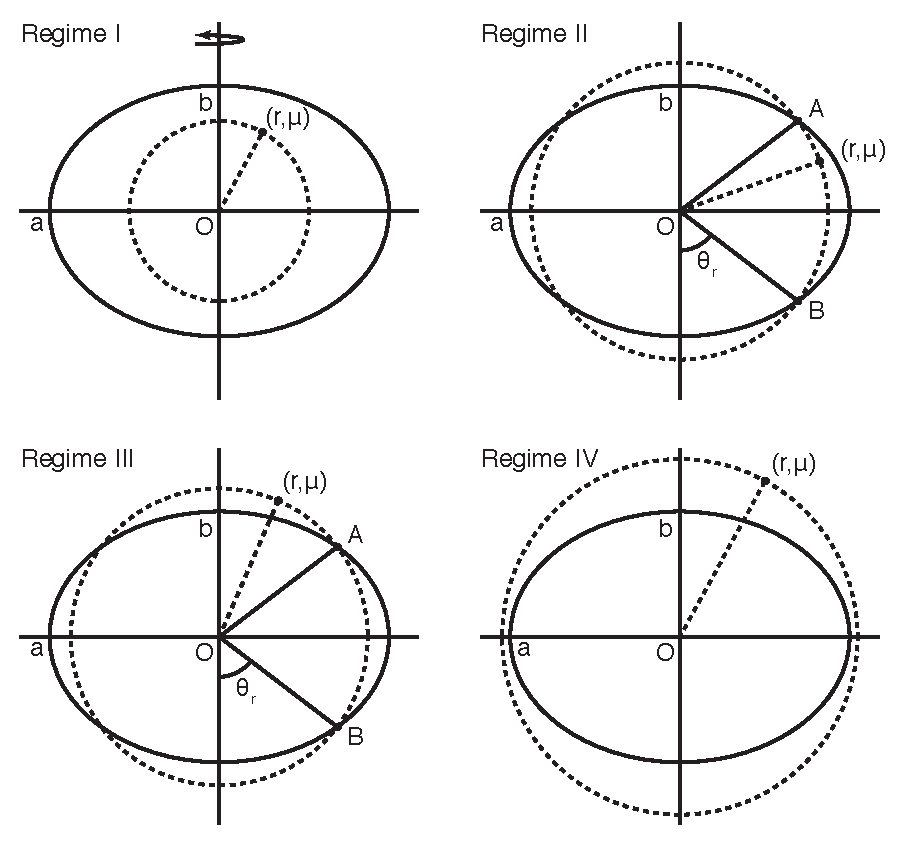
\includegraphics[scale=0.8333333]{Figures/HERCULES_regime_diagram2.pdf} 
   \caption{Schematic of the four regimes for calculating the potential of a constant density spheroid, see text for details. Black solid line shows a cross section through the spheroid, with the rotation axis vertical. The equatorial radius, $a$, and polar radius, $b$, are labeled. The point at which the potential is being evaluated, $(r,\mu)$, is marked by the point at the end of the dashed line. The dashed circle indicates the locus of all other points with a radius $r$ from the origin, O. The points on the spheroid where the radius of the surface is equal to $r$, i.e. $\tilde{r}(\mu)$ where $\mu$~$=$~$\pm \mu_r$, are labelled A and B.}
   \label{sup:fig:Regimes}
\end{figure*}


%%%%%%%%%%%%%%%%%%%%%%%%%%%%%%%%%
\subsubsection{Regime I: $r$~$\leq$~$b$}
\label{HUG:sec:R1}

The first regime is that for calculating the potential at a point within the spheroid, where the volume interior to the radius $r$ is all within the spheroid. 
This case was considered by \cite{Hubbard2013} but we rederive it here.
In this regime the potential is a sum of two terms: the first due to the mass within a sphere with radius $r$; and the second an integral over the mass in the ellipsoidal shell exterior to $r$.
Assuming that the body is axisymmetric and symmetrical relative to the equatorial plane, the potential function can be written as
%
\begin{align}
\begin{aligned}
{} & \Phi^I(r,\mu)= \frac{4\pi}{3} \rho G r^2 
 + 2\pi \rho G \int_{-1}^{1} \int_{r}^{\tilde{r} (\mu')} \left [ \sum_{l=0}^{\infty} \frac{r^{l}}{(r')^{l+1}} P_{l}(\mu)P_{l}(\mu') (r')^2 \mathrm{d}r' \right ] \mathrm{d}\mu' \,,
\end{aligned}
\end{align}
%
where $\rho$ is the density of the spheroid and $\tilde{r}(\mu)$ is the radius of the surface of the body at $\mu$.
Using the symmetry properties of the integrals, the expression simplifies to
%
\begin{align}
\begin{aligned}
{} & \Phi^I(r,\mu)=  4\pi \rho G \left \{ \frac{r^2}{3} \right. 
 \left. + \int_{0}^{1} \int_{r}^{\tilde{r}(\mu')} \left [ \sum_{k=0}^{\infty} \frac{r^{2k}}{(r')^{2k+1}} P_{2k}(\mu)P_{2k}(\mu') (r')^2 {\rm d}r' \right ] {\rm d}\mu' \right \} \,.
\end{aligned}
\end{align}
%
Now we integrate over the radial direction, considering the $k$~$=$~0,1 terms separately
%
\begin{align}
\begin{aligned}
 \Phi^I(r,\mu) =    4\pi \rho G  {} & \left \{ \frac{r^2}{3} \right .  \left . + \frac{1}{2} \int_{0}^{1} \left [ (\tilde{r}(\mu'))^2 - r^2 \right ] {\rm d}\mu' \right . \\
& \left. + r^2 P_{2}(\mu)  \int_{0}^{1} \left [ \ln \left ( \frac{\tilde{r}(\mu')}{r}\right ) P_{2}(\mu') \right ] {\rm d}\mu' \right . \\
& \left. + \sum_{k=2}^{\infty} \frac{r^{2k} P_{2k}(\mu)}{2-2k}  \int_{0}^{1} \left [ (\tilde{r}(\mu'))^{\, 2-2k} - r^{\, 2-2k} ) P_{2k}(\mu')  \right ] {\rm d}\mu'  \right \} \,.
\end{aligned}
\end{align}
%
This is similar in form to the expression found in \cite{Kong2013} for Regimes II and III. 
Therefore we use notation similar to that of \cite{Kong2013} and rewrite
%
\begin{align}
\begin{aligned}
\Phi^I(r,\mu) = \frac{4\pi}{3} \rho G r^2  {} & + \frac{G M}{r} \left [ \left ( \frac{r}{a} \right ) N_0(\xi, 1) \right. \left. -  \left ( \frac{r}{a} \right )^3 N_2(\xi,1) P_2(\mu) \right . \\
& \left . - \sum_{k=2}^{\infty}  \left ( \frac{r}{a} \right )^{2k+1} N_{2k}(\xi,1) P_{2k}(\mu) \right ] \,,
\end{aligned}
\end{align}
%
where
%
\begin{align}
\begin{aligned}
\label{HUG:eqn:1lay_M} 
M= \frac{4 \pi \rho}{3}  \int_{0}^{1} \left [ \tilde{r}(\mu') \right ]^3 {\rm d}\mu'  = \frac{4 \pi \rho}{3} a^3  \int_{0}^{1} \left [ \tilde{\xi}(\mu') \right ]^3 {\rm d}\mu' \,
\end{aligned}
\end{align}
%
is the mass of the spheroid,
%
\begin{align}
& \begin{aligned}
\label{HUG:eqn:1lay_N0}
N_0(\xi,\mu_r)  {} &=  \left (  \frac{3}{2} \right ) \frac{ \int_{0}^{\mu_r} \left [ (\tilde{\xi}(\mu'))^2 - \xi^2 \right ] {\rm d}\mu' }{\int_{0}^{1} \left [ \tilde{\xi}(\mu') \right ]^3 {\rm d}\mu' } \,, 
\end{aligned} \\[4ex]
%
& \begin{aligned}
\label{HUG:eqn:1lay_N1}
N_2(\xi,\mu_r) {} &= - \frac{ 3 \int_{0}^{\mu_r} \left [ \ln \left ( \tilde{\xi}(\mu') / \xi \right ) P_2(\mu') \right ] {\rm d}\mu' }{\int_{0}^{1} \left [ \tilde{\xi}(\mu') \right ]^3 {\rm d}\mu' } \,,
\end{aligned}
\end{align}
%
and
%
\begin{align}
& \begin{aligned}
\label{HUG:eqn:1lay_N2k}
N_{2k}(\xi,\mu_r) {} & =  -\left ( \frac{3}{2k-2} \right )  \frac{ \int_{0}^{\mu_r} \left [ \left ( \xi^{\, 2-2k} - (\tilde{\xi}(\mu'))^{\, 2-2k} \right ) P_{2k}(\mu') \right ] {\rm d}\mu' }{\int_{0}^{1} \left [ \tilde{\xi}(\mu') \right ]^3 {\rm d}\mu' }  \;\;\;   \textrm{for} \; k \ge 2 \,.
\end{aligned}
\end{align}
%
$\tilde{\xi}(\mu)$~$=$~$\tilde{r}(\mu)/a$ is the normalized radius on the surface of the body, $\xi$~$=$~$r/a$ is the normalized radius at which we are calculating the potential, and $a$ is the equatorial radius of the spheroid. We define $N_2$ with the opposite sign from that used in \cite{Kong2013} to be consistent with the definition of $N_{2k}$. This definition makes the expression for regimes II and III simpler.

The notation used here is similar to \cite{Kong2013}, but not exactly the same. \cite{Kong2013} use $\xi_0$~$=$~$r/a$ (which we denote $\xi$) and use $\xi(\mu)$ to denote the normalized radius at a point on the surface for which we have used $\tilde{\xi}(\mu')$.
We feel that the notation used in \cite{Kong2013} is confusing when considering multiple spheroids and so have adopted this new notation for clarity.

%%%%%%%%%%%%%%%%%%%%%%%%%%%%%%%%%
\subsubsection{Regime II: interior point with $b$~$<$~$r$~$<a$}
\label{HUG:sec:R2}

This case is the same as that considered by \cite{Kong2013}, but with the point at which the potential is being calculated within the body.
However, the location of the evaluation point relative to the surface does not change the expression for the potential in this regime and
%
\begin{align}
\begin{aligned}
 \Phi^{II}(r,\mu) = {}  & 2\pi \rho G \int_{-\mu_r}^{+\mu_r} \int_0^r \left [ \sum_{l=0}^{\infty} \frac{(r')^l}{r^{l+1}} P_l(\mu)P_l(\mu') (r')^2 {\rm d}r' \right ] {\rm d}\mu' \\
& + 2\pi \rho G \int_{-\mu_r}^{+\mu_r} \int_{r}^{\tilde{r}(\mu')} \left [ \sum_{l=0}^{\infty} \frac{r^l}{(r')^{l+1}} P_l(\mu)P_l(\mu') (r')^2 {\rm d}r' \right ] {\rm d}\mu' \\
& +2\pi \rho G \int_{\mu_r}^{1} \int_0^{\tilde{r}(\mu')} \left [ \sum_{l=0}^{\infty} \frac{(r')^l}{r^{l+1}} P_l(\mu)P_l(\mu') (r')^2 {\rm d}r' \right ] {\rm d}\mu' \\
& +2\pi \rho G \int_{-1}^{-\mu_r} \int_0^{\tilde{r}(\mu')} \left [ \sum_{l=0}^{\infty} \frac{(r')^l}{r^{l+1}} P_l(\mu)P_l(\mu') (r')^2 {\rm d}r' \right ] {\rm d}\mu' \,. 
\label{HUG:eqn:Kong15}
\end{aligned}
\end{align}
%
$\mu_r$~$=$~$cos\, \theta_r$ (Figure~\ref{sup:fig:Regimes}) is the value of $\mu$ for which the observation radius and the surface intersect, i.e. $\tilde{r}(\mu_r)$~$=$~$r$, in the upper hemisphere.
This can be integrated to give
%
\begin{align}
\begin{aligned}
\Phi^{II}(r,\mu) = \frac{G M}{r}  {} & \left \{ \left [ 1 - K_0(\xi, \mu_r) + \left ( \frac{r}{a} \right ) N_0 (\xi, \mu_r) \right ] \right . \\
& \left . - \sum_{k=1}^{\infty} \left [   \left (\frac{r}{a} \right )^{ \, 2 k + 1} N_{2k}(\xi, \mu_r) \right . \right. \left.\left.  + \left (\frac{a}{r} \right )^{2 k} (J_{2k}- K_{2k}(\xi, \mu_r) )\right ] P_{2k}(\mu) \right \} \,,
\label{HUG:eqn:RegII}
\end{aligned}
\end{align}
%
where
%
\begin{align}
& \begin{aligned}
\label{HUG:eqn:1lay_K0} 
K_0(\xi,\mu_r)  {} &=   \frac{ \int_{0}^{\mu_r} \left [ (\tilde{\xi}(\mu'))^3 - \xi^3 \right ] {\rm d}\mu' }{\int_{0}^{1} \left [ \tilde{\xi}(\mu') \right ]^3 {\rm d}\mu' } \,,
\end{aligned} \\[4ex]
%
& \begin{aligned}
\label{HUG:eqn:1lay_K2k} 
K_{2k}(\xi,\mu_r) {} &= - \left ( \frac{3}{2k+3} \right ) \frac{ \int_{0}^{\mu_r} \left [ \left ( (\tilde{\xi}(\mu'))^{\, 2k+3} - \xi^{\, 2k+3} \right ) P_{2k}(\mu') \right ] {\rm d}\mu' }{\int_{0}^{1} \left [ \tilde{\xi}(\mu') \right ]^3 {\rm d}\mu' }  \;\; \textrm{for}\; k \ge 1 \, ,
\end{aligned} 
\end{align}
%
and
%
\begin{align}
\label{HUG:eqn:1lay_J2k} 
J_{2k}  {} &=  - \left ( \frac{3}{2k+3} \right ) \frac{ \int_{0}^{1} \left [ (\tilde{\xi}(\mu'))^{\, 2k+3}  P_{2k}(\mu') \right ] {\rm d}\mu' }{\int_{0}^{1} \left [ \tilde{\xi}(\mu') \right ]^3 {\rm d}\mu' } \,.
\end{align}
%
$J_{2k}$ are the gravitational moments and are not dependent on $r$.
This is the same expression found by \citet{Kong2013}.

In dealing with single Maclaurin spheroids, \citet{Kong2013} could assume that 
%
\begin{align}
\mu_r=\frac{\sqrt{a^2-r^2}}{r \sqrt{\left (\frac{a}{b} \right )^2 -1}} \,.
\end{align}
%
For a general surface this is not the case and we find $\mu_r$ for each potential surface numerically.

%%%%%%%%%%%%%%%%%%%%%%%%%%%%%%%%%
\subsubsection{Regime III: exterior point with $b$~$<$~$r$~$<$~$a$}
\label{HUG:sec:R3}

This is the exact case that was considered by \cite{Kong2013}.
The expression in Equation~\ref{HUG:eqn:RegII} for the potential applies and $\Phi^{III}(r,\mu)$~$=$~$\Phi^{II}(r,\mu)$.

%%%%%%%%%%%%%%%%%%%%%%%%%%%%%%%%%
\subsubsection{Regime IV: $r$~$\geq$~$a$}
\label{HUG:sec:R4}

This regime was considered previously by \cite{Hubbard2012} and \cite{Kong2013}.
Since all the mass of the spheroid is interior to the evaluation point we need only consider a single term
%
\begin{align}
\label{sup:eqn:V4_1}
 \Phi^{IV} {} & (r,\mu)= 2\pi \rho G \int_{-1}^{1} \int_0^{\tilde{r}} \left [ \sum_{l=0}^{\infty} \frac{(r')^l}{r^{l+1}} P_l(\mu)P_l(\mu') (r')^2 {\rm d}r' \right ] {\rm d}\mu' \,.
\end{align}
%
Note that this expression in Equation 13 of \cite{Kong2013} is missing the $2\pi$ prefactor.
Integrating Equation~\ref{sup:eqn:V4_1} radially we get the expression
%
\begin{align}
\Phi^{IV}(r,\mu) {} &= \frac{G M}{r} \left [ 1-\sum_{k=1}^{\infty} \left ( \frac{a}{r} \right )^{2k} J_{2k} P_{2k}(\mu) \right ] \,,
\end{align}
%
which is the general expression for the potential outside of an axisymmetric body.


%%%%%%%%%%%%%%%%%%%%%%%%%%%%%%%%%%%%%%%%%%
%%%%%%%%%%%%%%%%%%%%%%%%%%%%%%%%%%%%%%%%%%
\subsection{The general concentric Maclaurin spheroid model}


\begin{figure}
\centering
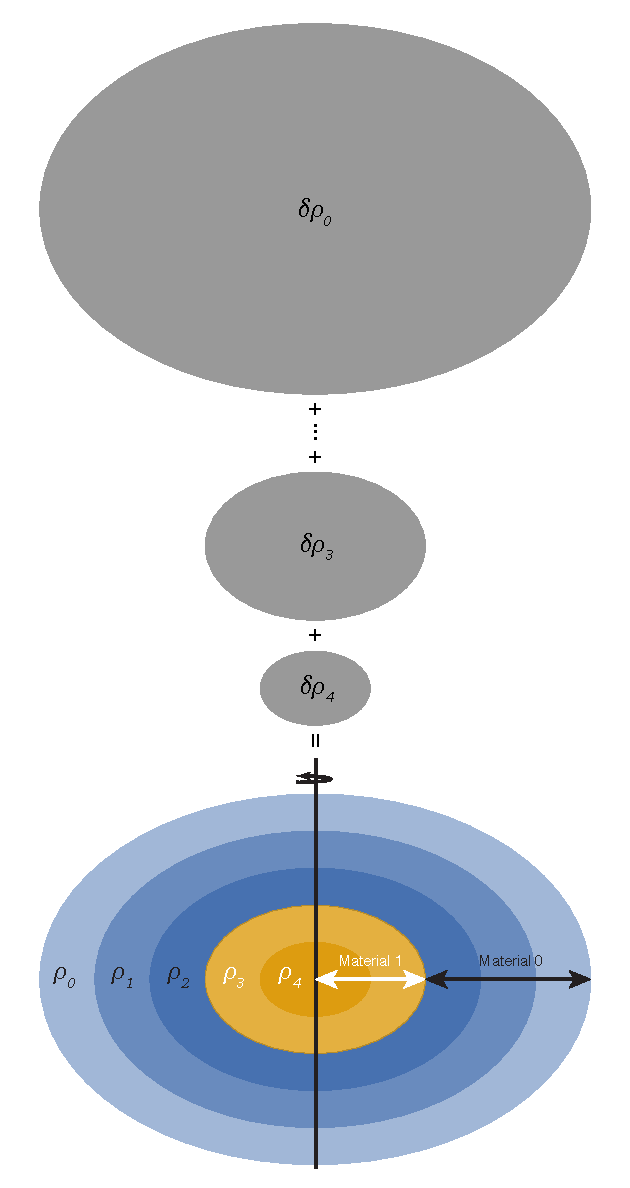
\includegraphics[scale=0.8333333]{Figures/HERCULES_schematic4.pdf}
\caption{Caption on next page.}
\end{figure}
%additional figure for caption
\setcounter{figure}{1}
\begin{figure}
\caption[]{Schematic of how an axisymmetric planetary structure is modeled in the HERCULES code. A body is described as a superposition of a number of constant-density spheroids of density $\delta\rho_{\rm i}$ (shown in gray). The superposition of the spheroids gives a body with increasing density with depth. The volumes between successive spheroids are called layers. Each layer has a constant density, $\rho_{\rm i}$, given by the sum of the densities of all the spheroids larger than the spheroid that defines the inner edge of the layer. Each layer belongs to a material layer which determines the relationship between pressure and total density in that layer by use of the material's equation of state. Two material layers are shown separately in blues and oranges. }
\label{HUG:fig:concentric_model}
\end{figure}



Now that we have expressions for the potential due to a single spheroid, we can now build on on the work of \cite{Hubbard2013} and develop a general model for a planet based on concentric Maclaurin spheroids.
After \cite{Hubbard2013} we consider modeling a planet as a number of uniform density layers made up of an array of $N_{\rm lay}$ nested spheroids (Figure~\ref{HUG:fig:concentric_model}).
The largest spheroid is numbered 0 and labels increase inwards. Layers are defined as the volume between two consecutive spheroids and are numbered by the spheroid that marks their outer surface.
The `real' densities of the layers, $\rho_i$, are given by the sum of the densities of each of the individual spheroids covering that layer. 
The density of each individual spheroid is therefore given by $\delta \rho_i = \rho_i - \rho_{i-1}$ for $i>0$ and $\delta \rho_0 = \rho_0$.
Conversely
%
\begin{align}
\rho_k=\sum_{i\leq k} \delta\rho_i \, .
\label{HUG:eqn:rho_sum}
\end{align}
%

The gravitational potential at any point is given by summing the gravitational potentials from each of the spheroids, accounting for fact that they are in different regimes:
%
\begin{align}
\Phi (r, \mu) = \sum_{i=0}^{i_{I}} \Phi^{I}_i (r, \mu) + \sum_{i=i_{I}+1}^{i_{IV}-1} \Phi^{II}_i (r, \mu) +  \sum_{i=i_{IV}^{N_{\rm lay}-1}} \Phi^{IV}_i (r, \mu) \, ,
\end{align}
%
where $i_{I}$ is the lowermost spheroid for which $r < b_i $, $i_{IV}$ is the uppermost spheroid for which $r > a_i $ and $N_{\rm lay}$ is the total number of spheroids.
Note that as regime II and III have the same expression for potential, we have combined both into regime II here. 

To calculate the equilibrium structure we solve for the position of the surfaces of the constant density spheroids, assuming they are equipotential surfaces. 
The radius of a point on the surface of the $i$th spheroid, $\tilde{r}_i(\mu)$, is then given by equating the potential at a point on the surface with the potential of that surface at the equator
%
\begin{align}
U (\tilde{r}_i(\mu), \mu) -U(a_i,0) = 0 \, ,
\end{align}
%
where $U=\Phi+Q$ is the total potential. The centrifugal potential, $Q$, for a corotating body is given by
%
\begin{align}
\begin{aligned}
 Q (r,\mu) =\frac{1}{3} r^2 \omega_{\rm rot}^2 \left [ 1 - P_2(\mu) \right ] \,,
 \end{aligned}
\end{align}
%
where $\omega_{\rm rot}$ is the corotating angular velocity. The total potential $U$ is given by summing the gravitational and centrifugal potentials i.e.,  $U$~$=$~$\Phi+Q$.

Combining our previous results, the equation that must be solved iteratively to find $\tilde{r}_j (\mu)$ is therefore
%
\begin{align}
\begin{aligned}
\label{HUG:eqn:all_start}
 \Phi(\tilde{r}_j(\mu), \mu) + Q(\tilde{r}_j(\mu), \mu)-\Phi(a_j,0) - Q(a_j,0) = 0 \,,
\end{aligned}
\end{align}
%
with
%
\begin{align}
& \begin{aligned}
\Phi (r, \mu) & = \sum_{i=0}^{i_{I}} \Phi^{I}_i (r, \mu) + \sum_{i=i_{I}+1}^{i_{IV}-1} \Phi^{II}_i (r, \mu) +  \sum_{i=i_{IV}}^{N_{\rm lay}-1} \Phi^{IV}_i (r, \mu) \,,
\end{aligned} \\[4ex]
%
& \begin{aligned}
\Phi_i^I(r,\mu){} & =  \frac{4\pi}{3} \delta\rho_i G r^2 + \frac{G M_i}{r} \left [ \left ( \frac{r}{a_i} \right ) N_{i,0}(\xi_i, 1) \right . \left . - \sum_{k=1}^{\infty}  \left ( \frac{r}{a_i} \right )^{2k+1} N_{i,2k}(\xi_i,1) P_{2k}(\mu) \right ] \,,
\end{aligned} \\[4ex]
%
& \begin{aligned}
\Phi^{II}_i(r,\mu) ={} & \frac{G M_i}{r} \left \{ \left [ 1 - K_{i,0}(\xi_i, \mu_{r,i}) + \left ( \frac{r}{a_i} \right ) N_{i,0} (\xi_i, \mu_{r,i}) \right ] \right .\\
& \left . - \sum_{k=1}^{\infty} \left [   \left (\frac{r}{a_i} \right )^{ \, 2 k + 1} N_{i,2k}(\xi_i, \mu_{r, i}) \right. \right. \left.  \left. + \left (\frac{a_i}{r} \right )^{2 k} (J_{i,2k}-K_{i,2k}(\xi_i, \mu_{r,i}) )\right ] P_{2k}(\mu) \right \} \,,
\end{aligned}
\end{align}
%
\begin{align}
& \begin{aligned}
\Phi^{IV}_i(r,\mu) {} &= \frac{G M_i}{r} \left [ 1-\sum_{k=1}^{\infty} \left ( \frac{a_i}{r} \right )^{2k} J_{i,2k} P_{2k}(\mu) \right ] \,,
\end{aligned} \\[4ex]
%
& \begin{aligned}
Q (r,\mu) =\frac{1}{3} r^2 \omega_{\rm rot}^2 \left [ 1 - P_2(\mu) \right ] \,,
\end{aligned} \\[4ex]
%
& \begin{aligned}
\label{HUG:eqn:Ni0}
N_{i,0}(\xi_i,\mu_r)  {} & = \left (  \frac{3}{2} \right ) \frac{ \int_{0}^{\mu_r} \left [ (\tilde{\xi_i}(\mu'))^2 - \xi_i^2 \right ] {\rm d}\mu' }{\int_{0}^{1} \left [ \tilde{\xi_i}(\mu') \right ]^3 {\rm d}\mu' } \,,
\end{aligned} \\[4ex]
%
& \begin{aligned}
\label{HUG:eqn:Ni2}
N_{i,2}(\xi_i,\mu_r) {} &= - \frac{ 3 \int_{0}^{\mu_r} \left [ \ln \left ( \tilde{\xi_i}(\mu') / \xi_i \right ) P_2(\mu') \right ] {\rm d}\mu' }{\int_{0}^{1} \left [ \tilde{\xi_i}(\mu') \right ]^3 {\rm d}\mu' } \,,
\end{aligned} \\[4ex]
%
& \begin{aligned}
\label{HUG:eqn:Ni2k}
N_{i,2k}(\xi_i,\mu_r) {} &=  -\left ( \frac{3}{2k-2} \right ) \frac{ \int_{0}^{\mu_r} \left [ \left ( \xi_i^{\, 2-2k} - (\tilde{\xi_i}(\mu'))^{\, 2-2k} \right ) P_{2k}(\mu') \right ] {\rm d}\mu' }{\int_{0}^{1} \left [ \tilde{\xi_i}(\mu') \right ]^3 {\rm d}\mu' } \;\; \textrm{for} \; k \ge 2 \,,
\end{aligned} \\[4ex]
%
& \begin{aligned}
\label{HUG:eqn:Ki0}
K_{i,0}(\xi_i,\mu_r)  {} &=  \frac{ \int_{0}^{\mu_r} \left [ (\tilde{\xi_i}(\mu'))^3 - \xi_i^3 \right ] {\rm d}\mu' }{\int_{0}^{1} \left [ \tilde{\xi_i}(\mu') \right ]^3 {\rm d}\mu' } \;\;,
\end{aligned} \\[4ex]
%
& \begin{aligned}
\label{HUG:eqn:Ki2k}
K_{i,2k}(\xi_i,\mu_r) {} &=  - \left ( \frac{3}{2k+3} \right ) \frac{ \int_{0}^{\mu_r} \left [ \left ( (\tilde{\xi_i}(\mu'))^{\, 2k+3} - \xi_i^{\, 2k+3} \right ) P_{2k}(\mu') \right ] {\rm d}\mu' }{\int_{0}^{1} \left [ \tilde{\xi_i}(\mu') \right ]^3 {\rm d}\mu' } \; \; \textrm{for} \; k \ge 1 \,,
\end{aligned} \\[4ex]
%
& \begin{aligned}
\label{HUG:eqn:Ji2k}
J_{i,2k}  {} &=  - \left ( \frac{3}{2k+3} \right ) \frac{ \int_{0}^{1} \left [ (\tilde{\xi_i}(\mu'))^{\, 2k+3}  P_{2k}(\mu') \right ] {\rm d}\mu' }{\int_{0}^{1} \left [ \tilde{\xi_i}(\mu') \right ]^3 {\rm d}\mu' } \,,
\end{aligned}
\end{align}
%
and
%
\begin{align}
& \begin{aligned}
\label{HUG:eqn:Mi}
M_i {} &= \frac{4 \pi \delta \rho_i a_i^3}{3}  \int_{0}^{1} \left [ \tilde{\xi_i}(\mu') \right ]^3 {\rm d}\mu' \,.
\end{aligned}
\end{align}
%
A subscript $i$ indicates the quantity was calculated for the $i$th spheroid. We define $\xi_i=r/a_i$, unlike \cite{Hubbard2013}, who normalizes all the $\xi$ to the equatorial radius of the outermost spheroid. $\mu_{r,i}=\mu_{r,i}(r)$ is different for each spheroid, $i$, and each point $r$.
Also note that the the $J_{i,2k}$ defined here for each spheroid are not the true gravitational moments as in \cite{Hubbard2013}, but scaled versions of the moments.
For a discussion of this see Section~\ref{HUG:sec:Js}.
These changes have been made to allow the spheroids to remain independent of each other for ease of calculation.

The Equations~\ref{HUG:eqn:all_start}-\ref{HUG:eqn:Mi} are much more complicated than in \cite{Hubbard2013} however they correctly account for all the different regimes for gravitational potential calculation and non-synchronous rotation. 
This will allow us to calculate the structure of rapidly rotating and super-CoRoL structures.

%%%%%%%%%%%%%%%%%%%%%%%%%%%%%%%%%%%%%%%%%%%%%%%%%%%%%
%%%%%%%%%%%%%%%%%%%%%%%%%%%%%%%%%%%%%%%%%%%%%%%%%%%%%
%%%%%%%%%%%%%%%%%%%%%%%%%%%%%%%%%%%%%%%%%%%%%%%%%%%%%
\section{Numeric Implementation}
\label{HUG:sec:numerics}

HERCULES iteratively solves for the equilibrium structure of a planet, modeling the body as a series of constant density, nested spheroids.
The code implements an algorithm to solve Equation~\ref{HUG:eqn:all_start} for a series of $N_\mu$ points on the surface of each spheroid, and uses the newly calculated equipotential surfaces to update the structure of the body. To make the iterative equation numerically tractable we truncate the series at a maximum spherical harmonic degree of $2k$~$=$~$2k_{\rm max}$.

The code can also iterate to conserve the mass of several material layers and the AM of the body.
The material layers (e.g. core, lower mantle, upper mantle etc.) are treated as real materials with equations of state (EOSs) that can be used to give self-consistent densities for each of the concentric layers.  Layers are defined as the material that exists in the volume bounded by the surfaces of two consecutive spheroids.
A layer is considered as being in a material layer if its outside surface is within or at the edge of that material layer.
Layers, spheroids, materials and material layers are numbered from the outside in, starting from $0$.
A summary of the nomenclature used in describing spheroids, layers, materials and material layers is given in the box below.
In this section, we outline the implementation of the iterative scheme in HERCULES and the various other features of the code. HERCULES is written using the C++ programming language.

%
\vspace{0.5cm}
\begin{tcolorbox}[colback=white, colframe=SchoolColor, title=Note on nomenclature]
In this user guide we use a number of different terms to describe features of the planetary structure.
Here we attempt to clarify the meaning of each of these.

\setlength{\parskip}{15pt}
\setlength{\leftskip}{1.5cm}
\setlength{\parindent}{-1.5cm}

{\it structure:} \newline
We use the term structure to describe the whole body/planet that is being calculated.

{\it spheroid} or {\it concentric spheroid:} \newline
This refers to one of the nested, concentric spheroids of density $\delta\rho_i$ that make up a planet in HERCULES. We use this term to refer to the whole spheroid.

{\it layer} or {\it concentric layer:} \newline
 This refers to the volume or mass between the surface of a spheroid and the surface of the spheroid beneath it. The density of each layer is given by the sum of the density of the spheroids that intersect the volume of that layer (Equation~\ref{HUG:eqn:rho_sum}). Layers are numbered corresponding to the spheroid that describes their outer surface.
 
 {\it surface} or {\it outer surface:} \newline
The surface of a given spheroid.

{\it material:} \newline The property of a layer that controls the relationship between pressure and density in that layer. For example, it could control the EOS used to calculate the density of that layer from the calculated pressure.

{\it material layer:} \newline  A material layer is the volume of the planet that is composed of a given material. 
The `real' density of the layers in this region are calculated in the same way, typically using the EOS of the relevant material using the calculated pressure.
A layer is considered to be part of a specific material layer if its outer surface lies within, or at the top of, the material layer.
Spheroids are not attached to a given material 
The actual mass of a given material has contributions from spheroids that are not considered part to be of that material layer as they have a volume that intersects the material layer.


\setlength{\leftskip}{0pt}
\setlength{\parskip}{0 pt}
\setlength{\parindent}{15pt}

\end{tcolorbox}

%%%%%%%%%%%%%%%%%%%%%%%%%%%%%%%%%%%%%%%%%%
%%%%%%%%%%%%%%%%%%%%%%%%%%%%%%%%%%%%%%%%%%
\subsection{Overview of algorithm}

Finding the equilibrium planetary structure in HERCULES is divided into a number of steps. 
Here, we outline the steps to provide a structure for discussing the different routines discussed below. 

\begin{enumerate}
\item {\bf Initialization:} This section reads in the input files and initializes the structure before the iteration routine begins. 
The root for this section is the \texttt{initialisation} function.
\begin{enumerate}[i.]
%
\item {\bf Read input:} The input file is read in and from it the lengths of various vectors are defined. 
This is done in the \texttt{read\_input} function. 
This function also defines the material layers and reads in the EOS files.
For a discussion of the input file see Section~\ref{HUG:sec:input}. 
%
\item \label{item:init} {\bf Initialize the structure:} Next, an initial approximation of the planet's structure is made.
This can be done assuming a single density for all spheroids, a constant density body or by reading in a binary output file (see Section~\ref{HUG:sec:init}).
%
\item {\bf Calculate structure properties:} Calculate various properties of the structure. 
This includes: the precomputed integrals (see Section~\ref{HUG:sec:precalc}); the mass, AM, gravitational moments and moments of inertia for each spheroid \\\noindent(\texttt{concentric\_layer.calc\_M}, \texttt{planet.calc\_Mtot},  \texttt{planet.calc\_Ltot}, \\\noindent \texttt{concentric\_layer.calc\_Js} and \\ \noindent \texttt{concentric\_layer.calc\_I}); and the potential at the equator of each spheroid.
With the exception of the latter, the calculation of these properties is done in the routine for initializing the structure in Section~\ref{item:init}. The initial structure is output to a binary file.
\end{enumerate}
%%
%%
\item {\bf Iteration:} The main body of the code is a single iteration to find the equilibrium structure with two nested iterations for calculating the shape of each of the spheroids and controlling the mass and AM of the body. 
A schematic of the iteration is given in Figure~\ref{HUG:fig:algorythm} and we will describe the main steps below. 
The root for the iteration section of the code is the function \texttt{iterate}.
\begin{enumerate}[i.]
%
\item {\bf Shape iteration:} The shape of the equipotential surfaces, corresponding to the potential at the equator of each of the spheroids from the previous iteration/initialization, is found. 
A Newton-Raphson method is used to find the $\xi_i$ point corresponding to the solution for Equation~\ref{HUG:eqn:all_start} at each $\mu_i$ point on each surface (see Section~\ref{HUG:sec:shape}).
The gradient of the function given in Equation~\ref{HUG:eqn:all_start} is determined numerically, calculating the potential at $\xi$ points separated by $\delta \xi$ to calculate the gradient of the function given in .
This process is repeated for all the surface points.
The structure of the body is kept constant throughout this process and only updated in the next step. 
%
\item {\bf Update planetary structure:} The structure of the planet is changed so that the surface of the spheroids correspond to the equipotential surfaces calculated in the shape iteration.
By definition, changing the shape of the spheroids changes the equipotential surfaces, but over several iterations the shape of the structure will converge.
The structure-specific precomputed integrals are recalculated (Section~\ref{HUG:sec:precalc}) along with the mass, AM, gravitational moments and moments of inertia for each spheroid and the total potential at the equator of each spheroid. 
%
\item {\bf Mass and AM control iteration:} Routines for controlling the mass and AM are applied (see Sections~\ref{HUG:sec:Mconc} and \ref{HUG:sec:AMconc}).
The AM control routine is performed after the mass control routine.
After each, if properties of the structure have changed, the relevant properties and precomputed integrals are recalculated.
The routines are looped over until a convergence criteria is met (see Section~\ref{HUG:sec:convergence}). Both control routines are performed in each iteration.
%
\item {\bf Access convergence:} The final step is to access whether the convergence criterion for the whole iteration has been met (see Section~\ref{HUG:sec:convergence}).
The previous three steps are repeated until either the convergence criteria are met or a maximum number of iterations is reached.
\end{enumerate}

\item {\bf Output:} The final structure is output to a binary file. A file containing the initial structure is also output at the end of the initialization step, and additional files can be output at the end of each full iteration.
\end{enumerate}

\clearpage
\begin{figure}[]
   \centering
   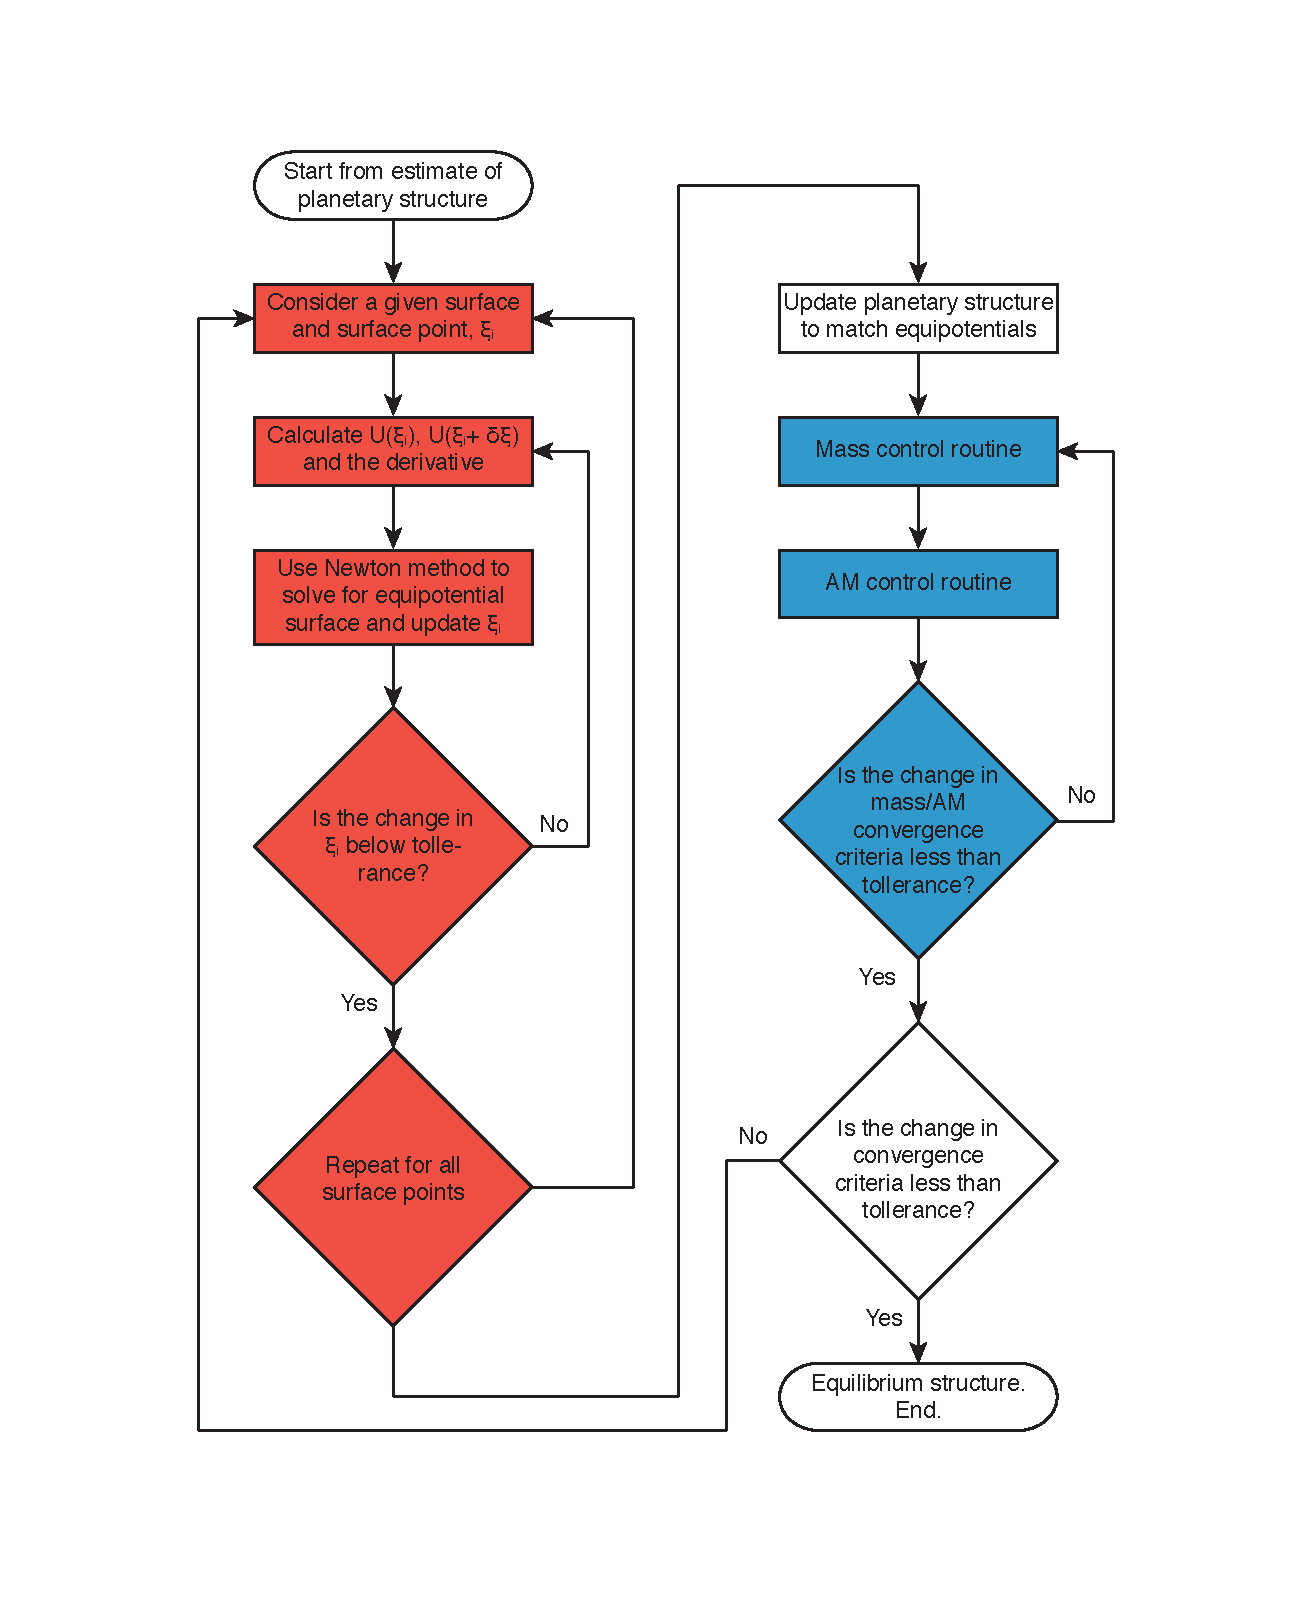
\includegraphics[width=0.85\textwidth, trim={3cm 2.5cm 3cm 2.5cm },clip]{Figures/HERCULES_algorythm2.pdf} 
   \caption{Outline of HERCULES algorithm. Red indicates the shape iteration and blue the mass and AM control iteration.}
   \label{HUG:fig:algorythm}
\end{figure}


%%%%%%%%%%%%%%%%%%%%%%%%%%%%%%%%%%%%%%%%%%
%%%%%%%%%%%%%%%%%%%%%%%%%%%%%%%%%%%%%%%%%%
\subsection{Initialization}
\label{HUG:sec:init}

HERCULES allows for two different ways of initializing a structure, either assuming a constant density for all spheroids or from a HERCULES binary output file.
The choice of initialization procedure is made by the use of the start flag, $\mathcal{F}_{\rm start}$, in the input file (see Section~\ref{HUG:sec:input}).
 
%%%%%%%%%%%%%%%%%%%%%%%%%%%%%%%%%
\subsubsection{Constant density spheroids: $\mathcal{F}_{\rm start}=0$}
This procedure (in \texttt{planet.initialise\_ellipsoids} called from \texttt{initialisation}) initializes the structure as nested Maclaurin spheroids.
The surfaces are equally spaced in equatorial radius within each material layer. The number of layers in each material, $N_{\rm lay}^{\rm mat}$, and the initial equatorial radii for each material layer, $a_{\rm mat}$, are given in the input file. 
The shape of the spheroids is dictated by the initial aspect ratio, $\mathcal{A}=b/a$, given in the input file.
The surface points on each ellipsoid are given by
%
\begin{align}
\xi_i(\mu_j)^2=\frac{b_i^2}{\left(a_i\mu_j\right)^2 + b_i^2 \left (1 - \mu_j \right)^2} \, .
\end{align}
%

The density of the spheroids is set depending on the mass control flag.
For constant density layers ($\mathcal{F}_{\rm Mconc}=0$) the density of the layers is set to the reference density, $\rho_{\rm ref}$, given in the input file.
For all other routines, the density is calculated so that each material layer has the desired mass, with each spheroid in each material layer having the same density.
The mass in a layer is given by the sum of the mass of all the spheroids covering the region with that material:
%
\begin{align}
\begin{aligned}
M_{k} ^{\rm mat}=\sum_{i<k}^{\rm material} \delta\rho_i \sum_{j:i}^{\rm layers} (V_{\rm out}^k - V_{\rm in}^k) + \delta\rho_k \sum_{i:k}^{\rm layers}  (V_{i} - V_{in}^k) \, ,
\end{aligned}
\end{align}
%
where $M_k^{\rm mat}$ is the mass of material $k$, $V_{\rm out}^k$ and $V_{\rm in}^k$ are the volume of the outside and inside layers of material $k$, and $\delta\rho_i$ is the constant density for spheroids in material $i$. $i:k$ indicates the layers that are of material $k$.
This can be rearranged to give the density of spheroids in material layer $k$
%
\begin{align}
\begin{aligned}
\delta\rho_k  = \frac{M_{k}^{\rm mat} -\sum_{i<k}^{\rm material} \delta\rho_i \sum_{j:i}^{\rm layers} (V_{\rm out}^k - V_{\rm in}^k)}{\sum_{i:k}^{\rm layers} (V_{i} - V_{\rm in}^k)} \, .
\end{aligned}
\end{align}
%
The density for spheroids in each material layer can then be found, working from the outermost material inwards. 

This routine also initializes a constant rotation for each layer.
If $\mathcal{F}_{\rm Lconc}=0$ then the rotation rate is set to be that given in the input file; otherwise a constant rotation rate that satisfies AM conservation is set.
This can be later overruled depending on the AM control routine used.

%%%%%%%%%%%%%%%%%%%%%%%%%%%%%%%%%
\subsubsection{From an output file: $\mathcal{F}_{\rm start}=1$}
The structure can also be initialized by reading in a HERCULES binary output file whose file location is given in the input file.
This is done in the \texttt{initialisation} function.
The shape, thermodynamic properties and rotational state of the structure are set to be the same as the given start file. $k_{\rm max}$, material EOSs, target mass and AM, $p_{\rm min}$, and run parameters are all maintained from the original input file. 
The properties of the planet are then recalculated within the code to ensure consistency. 

%
\vspace{0.5cm}
\begin{tcolorbox}[colback=white, colframe=SchoolColor, title=Note]
At present, the body in the start file is required to have the same $N_{\rm lay}$, $N_{\rm mat}$, $N_{\rm lay}^{\rm mat}$ and $N_{\mu}$ as defined in the input file for the present run.
\end{tcolorbox}

%%%%%%%%%%%%%%%%%%%%%%%%%%%%%%%%%%%%%%%%%%
%%%%%%%%%%%%%%%%%%%%%%%%%%%%%%%%%%%%%%%%%%
\subsection{Shape iteration}
\label{HUG:sec:shape}

The shape iteration takes each $\mu_j$ point on a surface in turn and, using a Newton-Raphson method, solves Equation~\ref{HUG:eqn:all_start} to find the location of the equipotential surface corresponding to the potential at the surface of that spheroid at the equator.
This routine is in the function \texttt{itterate}.
The equation this routine is solving is Equation~\ref{HUG:eqn:all_start} for a specific $\mu_j$:
%
\begin{align}
 X(\tilde{r}_i(\mu_j), \mu_j)= \Phi(\tilde{r}_i(\mu_j), \mu_j) + Q(\tilde{r}_i(\mu_j), \mu_j)-\Phi(a_i,0) - Q(a_i,0) = 0 \, .
 \end{align}
%
The current surface of spheroid $i$ is used as an initial guess to the position of the equipotential surface, i.e., $\xi_i^0=\tilde{\xi}_i(\mu_j)$.
The value of the function $X$ is calculated at a point $\xi_i$ and a point $\xi_i+\delta\xi$, to numerically determine the gradient of the function. $\delta\xi$ is defined by the user.
The approximation to the equipotential surface is then updated using the Newton-Raphson formula with a first order determination of the $X$ function gradient
%
\begin{align}
\xi_i^{n+1}=\xi_i^n-\frac{X(\xi_i^n, \mu_j) \delta\xi}{X(\xi_i^n+\delta\xi, \mu_j)-X(\xi_i^n, \mu_j)} \, .
\end{align}
%
The iteration continues with new determinations of $X$ until the convergence criteria are met (see Section~\ref{HUG:sec:convergence}).


\vspace{0.5cm}
\begin{tcolorbox}[colback=white, colframe=SchoolColor, title=Note]
While the equipotential surfaces are found, the structure used to calculate the gravitational and rotational potential is not changed. 
\end{tcolorbox}


%%%%%%%%%%%%%%%%%%%%%%%%%%%%%%%%%%%%%%%%%%
%%%%%%%%%%%%%%%%%%%%%%%%%%%%%%%%%%%%%%%%%%
\subsection{Thermodynamics and equations of state}
\label{HUG:sec:thermo}

In HERCULES, there are options to treat the concentric layers as being made of a real material with a defined EOS. 
Generally this is done in the mass control routines that change the density of a layer depending on the pressure and material within that layer (see Section~\ref{HUG:sec:Mconc}).
In the following sections we outline how the pressure of a given layer is calculated from the equatorial potential and density, and then describe the structure of the EOSs that HERCULES can use. 

%%%%%%%%%%%%%%%%%%%%%%%%%%%%%%%%%
\subsubsection{Calculation of pressure}
\label{HUG:sec:press_calc}

The pressure in the structure is calculated assuming hydrostatic equilibrium. 
Given that each of the layers is of constant density, the pressure at the top of a layer can be calculated as follows \citep{Hubbard2013}:
%
\begin{align}
\label{HUG:eqn:press}
p_i=p_{i-1}+\rho_{i-1}\left[ U(a_i, 0) - U(a_{i-1}, 0) \right ] \,.
\end{align}
%
In HERCULES, the pressure at the surface of the outermost spheroid is specified, $p_0=p_{\rm min}$, and so the pressure at the top of all subsequent layers can be determined sequentially.
The pressure at the centre of the body is given by
%
\begin{align}
p_{\rm core}=p_{N_{\rm lay}-1}+\rho_{N_{\rm lay}-1}\left[ U(0, 0) - U(a_{N_{\rm lay}-1}, 0) \right ]\,.
\end{align}
%
which is calculated for reference and used for some convergence criteria (see Section~\ref{HUG:sec:convergence}).

To calculate the density, we use an approximation for the pressure in the middle of the layer by taking the average of the pressure at the top and bottom of the layer. 
This approximation amounts to assuming that the variation in potential is linear within each layer.
The assumption of linear potential is a reasonably good one in most cases. 

%%%%%%%%%%%%%%%%%%%%%%%%%%%%%%%%%
\subsubsection{Equations of state}

In this version of HERCULES, equations of state must have a common structure, although future versions will allow for more EOS types.
HERCULES accepts EOS as ASCII files with columns of pressure, density, temperature and entropy (although the latter two are not used in calculations or indeed stored for the structure).  
For the structure of these files see Section~\ref{HUG:sec:input}. Any monotonically increasing density profile is allowable, but the $p$-$\rho$ relationships are defined at runtime so properties like total energy are not conserved.
Future versions of HERCULES will allow for the calculation of thermal structure within the code to conserve such properties.

In order to calculate the density from a given pressure, the EOS function \texttt{calc\_rho} linearly interpolates the given $p$-$\rho$ points.
There is also an option (see Section~\ref{HUG:sec:output}) to interpolate the points linearly in log space for densities below 3000~kg~m$^{-3}$, which may give better results in the the low density regime. 

%%%%%%%%%%%%%%%%%%%%%%%%%%%%%%%%%%%%%%%%%%
%%%%%%%%%%%%%%%%%%%%%%%%%%%%%%%%%%%%%%%%%%
\subsection{Mass control}
\label{HUG:sec:Mconc}

HERCULES contains a number of different routines to alter the density of spheroids to control the mass of each material layer.
Typically these routines attempt to conserve the mass in each material layer, and are applied in the mass/AM iteration after the shape iteration and are in the \texttt{itterate} function.
The properties of the planet are recalculated after mass control.

%%%%%%%%%%%%%%%%%%%%%%%%%%%%%%%%%
\subsubsection{Constant density: $\mathcal{F_{\rm Mconc}}=0$}

This option does not alter the density of the spheroids and keeps them constant throughout the calculation. 
If $\mathcal{F_{\rm start}}=0$, the density of each concentric layer is set to the reference density, $\rho_{\rm ref}$, at the start of the calculation.
Note that this mass control option is not compatible with any AM conservation routine and only works for an imposed, constant rotation rate: AM control routine option $\mathcal{F_{\rm Lconc}}=0$ (Section~\ref{HUG:sec:AMconc}).
This routine does not conserve the mass of the body or of material layers.

%%%%%%%%%%%%%%%%%%%%%%%%%%%%%%%%%
\subsubsection{Density scaling: $\mathcal{F_{\rm Mconc}}=1$}

This option allows the mass of the body to be conserved by scaling the density of each spheroid.
The density is determined from the EOS for the relevant material using the calculated pressure. The densities of all layers in a given material are then scaled by a constant factor that conserves the mass of that material.
The scaling factors, $\lambda_i$, depend on each other as conserving the mass in one material layer requires knowledge of the density of all concentric spheroids that have a volume that intersects part of the volume of the material layer.
After scaling, the mass of a given material $k$ is given by
%
\begin{align}
\begin{aligned}
M_{k}^{\rm mat} =\sum_{i<k}^{\rm material} \lambda_i \sum_{j:i}^{\rm layers}  \delta \rho_j (V_{\rm out}^k - V_{\rm in}^k) +\sum_{i:k}^{\rm layers} \rho_i \lambda_k (V_{i} - V_{\rm in}^k) \, ,
\end{aligned}
\end{align}
%
where $M_k^{\rm mat}$ is the mass of material layer $k$, $V_{\rm out}^k$ and $V_{\rm in}^k$ are the volume of the outside and inside spheroids, and $\lambda_k$ is the density scaling factor for material $k$. $i:k$ indicates the layers that are of material $k$.
We can rewrite this to give
%
\begin{align}
\begin{aligned}
\lambda_k = \frac{M_{k}^{\rm mat} -\sum_{i<k}^{\rm material} \lambda_i \sum_{j :i}^{\rm layers}  \delta\rho_j (V_{\rm out}^k - V_{\rm in}^k) }{\sum_{i:k}^{\rm layers} \delta\rho_i  (V_{i} - V_{\rm in}^k)} \, ,
\end{aligned}
\end{align}
%
which can be solved sequentially for each $\lambda_k$, starting from the outermost material layer. 
In this way, we require no prior knowledge of the other $\lambda_k$ that are yet to be determined. 

The change in the density also feeds back to a change in the pressure structure and hence calculated densities. 
The routine is therefore iterated over as part of the mass and AM control iteration until the convergence criteria are met (see Section~\ref{HUG:sec:convergence}). 

This density scaling preserves the mass of the body, but results in a distortion of the EOS for each material.
This was the approach taken by \cite{Hubbard2013}, as for Jupiter the radius of the planet is better determined than the EOS of helium-hydrogen mixtures. 
However, for other application the distortion of the EOS may not be acceptable. 

%%%%%%%%%%%%%%%%%%%%%%%%%%%%%%%%%
\subsubsection{Volume scaling: $\mathcal{F_{\rm Mconc}}=2$}

HERCULES can also conserve the mass of the planet by using a consistent EOS but by scaling the radius of the material layers. 
For this routine the density of each layer is determined from the pressure and the EOS only.
The equatorial radius of each spheroid in a material is then scaled by a constant factor to maintain the mass of that material layer.
As for the previous routine, we calculate the required scaling factors by considering the mass of a material layer after scaling:
%
\begin{align}
\begin{aligned}
M_{k}^{\rm mat} =\sum_{i<i_{\rm out}^k} \delta\rho_i(\lambda_k V_{\rm out}^k -\lambda_{k+1} V_{\rm in}^k) +\sum_{i_{\rm out}^k\le i<i_{\rm in}^k} \delta \rho_i(\lambda_k V_{i} -\lambda_{k+1} V_{\rm in}^k) \, ,
\end{aligned}
\end{align}
%
where $M_k^{\rm mat}$ is the mass of material layer $k$, $i_{\rm out}$ is the index of the outermost layer in material layer $k$, $i_{\rm in}^k$ is the index of the shell on the inside boundary of material layer $k$ (note that this layer is not of  material $k$), $V_{\rm out}^k$ and $V_{\rm in}^k$ are the volume of the outside and inside spheroids, and $\lambda_k$ is the volume scaling factor for material $k$ which applies to the volume of the spheroids inside material layer $k$. 
Rewriting this expression:
%
\begin{align}
\begin{aligned}
M_{k}^{\rm mat} = \lambda_k \left ( \sum_{i<i_{\rm out}^k} \delta\rho_i  V_{\rm out}^k +\sum_{i_{\rm out}^k\le i<i_{\rm in}^k} \rho_i V_{i}\right )  -\lambda_{k+1} \left ( \sum_{i<i_{\rm out}^k} \delta\rho_i V_{\rm in}^k +\sum_{i_{\rm out}^k\le i<i_{\rm in}^k} \rho_i V_{\rm in}^k \right ) \, ,
\end{aligned}
\end{align}
%
which can be rearranged to give
%
\begin{align}
\begin{aligned}
 \lambda_k = \frac{ M_{k}^{\rm mat}+ \lambda_{k+1} \left ( \sum_{i<i_{\rm in}} \rho_i V_{\rm in}^k  \right )}{ \left ( \sum_{i<i_{\rm out}} \rho_i  V_{\rm out}^k +\sum_{i_{\rm out}\le i<i_{in}} \rho_i V_{i}\right ) } \, .
\end{aligned}
\end{align}
%
We can then solve for each $\lambda_{k}$ sequentially from the inside out, as for the innermost material
%
\begin{align}
\begin{aligned}
 \lambda_{N_{\rm mat}-1}= \frac{ M_j^{\rm mat}}{ \left ( \sum_{i<i_{\rm out}^{j}} \rho_i  V_{\rm out}^{j} +\sum_{i_{\rm out}^j\le i<i_{\rm in}^j} \rho_i V_{i}\right ) } \,,
\end{aligned}
\end{align}
%
where $j=N_{\rm mat}-1$, which requires no prior knowledge of the other $\lambda$.

The volume scaling is applied by scaling the equatorial radius, $a$.
The scaled $a_i$, $a_i'$, are given by 
%
\begin{align}
\begin{aligned}
a'=\lambda^{\frac{1}{3}} a \,.
\label{HUG:eqn:a_scaling}
\end{aligned}
\end{align}
%
Each of the spheroids in the body are then given the new scaled equatorial radii, and hence polar radii, but their shape remains unchanged. 
This routine conserves mass but must be iterated over to give density and pressure profiles that are consistent with the EOS.

In some cases, the difference in scaling factors between material layers causes the surface of spheroids to change radial order i.e., $a_{i-1}$ can be less than $a_{i}$. 
Such an arrangement is not acceptable in HERCULES.
The radii of any crossing spheroids are altered sequentially from the outside inwards so that
%
\begin{align}
a_i=a_i'+1.005 \times (a_i'-a_{i-1}') \,.
\end{align}
%
where $a_i'$ are the equatorial radii calculated from scaling the spheroids as described above.
A single crossing surface can cause several spheroids to have their radii altered which is done sequentially from the outside inwards.

Similarly, the routine ensures there are not large gaps between the surface of spheroids at the contact between material layers. 
If the gap between the outermost layer of one material and the innermost layer of the next is greater than 5\% more than the  spacing in the upper material, the equatorial radii of spheroids whose surfaces are in the upper material layer are altered. 
The radii of all the relevant spheroids are decreased such that the gap between the bounding spheroids is the same as the spacing of spheroids in the upper layer.

When the radii of the spheroids must be changed from their calculated positions from Equation~\ref{HUG:eqn:a_scaling}, mass is not conserved on that iteration step. 
Over several iterations the structure will come to an arrangement where radii scaling corrections are not necessary and mass conservation is achieved.

%%%%%%%%%%%%%%%%%%%%%%%%%%%%%%%%%%%%%%%%%%
%%%%%%%%%%%%%%%%%%%%%%%%%%%%%%%%%%%%%%%%%%
\subsection{Angular momentum control}
\label{HUG:sec:AMconc}

HERCULES has a number of routines to control the rotational state of a planet. 
These routines are applied after the mass control routines.
Since the rotational state feeds back into the structure of the planet, the AM control routines are iterated over, along with the mass control routines, to acquire a self consistent structure.

\vspace{0.5cm}
\begin{tcolorbox}[colback=white, colframe=SchoolColor, title=Note]
In the current version of HERCULES, each layer has a constant rotational velocity, $\omega$, but this will be altered in future versions.
\end{tcolorbox}


%%%%%%%%%%%%%%%%%%%%%%%%%%%%%%%%%
\subsubsection{No conservation with constant rotation rate: $\mathcal{F}_{\rm Lconc}=0$}

When using this flag, the rotational profile of the planet is not changed during the calculation.
For $\mathcal{F}_{\rm start}=0$ the body is set as corotating with the angular velocity given in the input file.
For $\mathcal{F}_{\rm Lconc}=1$ the angular velocity of each of the layers is kept constant from the initial structure.


%%%%%%%%%%%%%%%%%%%%%%%%%%%%%%%%%
\subsubsection{Angular momentum conservation with imposed $\omega$ profile: $\mathcal{F}_{\rm Lconc}=1$}

This routine conserves AM by prescribing a given angular velocity profile. In potential theory, a conserved field is achieved only if the angular velocity is purely a function of distance from the rotation axis. In the current version of HERCULES, each layer has its own rotation rate. To have a conservative field each layer must have the same angular velocity. However, while iterating to find the equilibrium structure, the angular velocity of the body may exceed the angular velocity of a Keplerian orbit at the equator, i.e., the body may exceed the CoRoL. A super-Keplerian angular velocity leads to negative pressure gradients in the structure which breaks the requirement for a monotonically decreasing density with radius. It is hence helpful to allow the outer layers of the structure to be on sub-Keplerian orbits at intermediate iteration steps to allow the iteration to continue, as long as the final body is corotating. Otherwise, the structure of the final body is not accurately determined using a potential field method. 

The form of the profile used for this routine is that of a corotating planet and a sub-Keplerian outer region.
The angular velocity of each layer is prescribed as:
%
\begin{align}
\begin{aligned}
\omega=\min(\omega_{\rm orb}, \omega_{\rm rot}) \,,
\end{aligned}
\end{align}
%
where $\omega_{\rm orb}$ is the angular velocity of a particle in pressure supported keplerian orbit and $\omega_{\rm rot}$ is the angular velocity of the corotating body. 
In theory, $\omega_{\rm orb}$ is given by balancing the centrifugal force with the pressure gradient and the gravitational potential gradient in the equatorial plane
%
\begin{align}
\begin{aligned}
\mathrm{acceleration}=-\omega_{\rm orb}^2 r = -\frac{1}{\rho} \frac{\partial p}{\partial r} + \frac{\partial \Phi}{\partial r} \, .
\end{aligned}
\end{align}
%
Solving for $\omega_{\rm orb}$ gives
%
\begin{align}
\begin{aligned}
\omega_{\rm orb} = \sqrt{\frac{1}{r} \left [ \frac{1}{\rho} \frac{\partial p}{\partial r} - \frac{\partial \Phi}{\partial r} \right ] } \,.
\end{aligned}
\end{align}
%
However, the expression above for $\omega_{\rm orb}$ is effectively the same expression we use to enforce hydrostatic equilibrium in the structure (Equation~\ref{HUG:eqn:press}). 
The structure that satisfies conservation of AM is non-unique and, for this routine, we impose the orbital angular velocity profile to fully constrain the problem.


We define the orbital velocity by forcing it to be a fraction of the keplerian velocity that varies with radius
%
\begin{align}
\begin{aligned}
\omega_{\rm orb}=f \omega_{\rm kep} = f \sqrt{\frac{1}{r} \left [  - \frac{\partial \Phi}{\partial r} \right ] } \,,
\end{aligned}
\end{align}
%
where 
%
\begin{align}
\begin{aligned}
f = \Omega_1- \Omega_2 \left (1 - \frac{r_{eq}}{a_0} \right ) ^{\Omega_3} \,,
\end{aligned}
\end{align}
%
and $r_{eq}$ is the radius in the equatorial plane and $\Omega_i$ are user defined constants. 
Note that as $r_{eq} \rightarrow a_0$, $f\rightarrow \Omega_1$ and as $r_{eq} \rightarrow 0$, $f\rightarrow \Omega_1- \Omega_2$.
To calculate the structure of a body that is corotating except when it exceeds the CoRoL, set $\Omega_1=1$ and $\Omega_{2}=0$.
Having defined $\omega_{\rm orb}$, the only free parameter we have now is $\omega_{\rm rot}$ which can be solved for by conserving AM.

To find $\omega_{\rm rot}$, we conserve AM, but to do this we need to know the moments of inertia of each layer and hence each spheroid.
The moment of inertia about the $z$ axis of the $i$th constant-density spheroid is defined as
%
\begin{align}
\begin{aligned}
I_i=\int_{\mathcal{V}} \frac{2}{3} \delta \rho_i r^2 (1-P_2(\mu)) \mathrm{d}V' \,,
\end{aligned}
\end{align}
%
or alternatively
%
\begin{align}
\begin{aligned}
I_i=\frac{4 \pi}{3} \delta \rho_i  \int_{-1}^{1} \int_0^{\tilde{r_i}(\mu')} (r')^4 (1-P_2(\mu')) \mathrm{d}r' \mathrm{d}\mu' \,.
\end{aligned}
\end{align}
%
We use the symmetry of the spheroids and integrate over $r$ to give
%
\begin{align}
\begin{aligned}
I_i=\frac{8 \pi}{15} \delta \rho_i  \int_{0}^{1}  (\tilde{r_i}(\mu'))^5 (1-P_2(\mu')) \mathrm{d}\mu' \,.
\end{aligned}
\end{align}
%
This is the expression for the moment of inertia for a given spheroid. 

Each layer in HERCULES has a constant angular velocity.
We need to know the moment of inertia for each layer between two spheroids to calculate the AM.
Consider the moment of inertia of the material in the $i$th spheroid that lies between the surfaces of the smaller spheroids $n$ and $j$.
In this case the moment of inertia of the material in layer $i$ that lies between spheroids $n$ and $j$ is
%
\begin{align}
\begin{aligned}
I_{n\rightarrow j, i}=\frac{4 \pi}{3} \delta \rho_i  \int_{-1}^{1} \int_{\tilde{r}_{j}(\mu')}^{\tilde{r}_n(\mu')} (r')^4 (1-P_2(\mu'))\mathrm{d}r' \mathrm{d}\mu'  \,.
\end{aligned}
\end{align}
%
We use the symmetry of the spheroids and integrate over $r$ to give
%
\begin{align}
\begin{aligned}
I_{n\rightarrow j,i}=\frac{8 \pi}{15} \delta \rho_i  \int_{0}^{1}  \left [ (\tilde{r}_n(\mu'))^5 -\tilde{r}_j(\mu'))^5 \right ] (1-P_2(\mu')) \mathrm{d}\mu' \,.
\end{aligned}
\end{align}
%
This is simply
%
\begin{align}
\begin{aligned}
I_{n\rightarrow j,i}=\frac{\delta\rho_i}{\delta\rho_n} I_n - \frac{\delta\rho_i}{\delta\rho_j} I_j \,,
\end{aligned}
\end{align}
%
where $i\leq n<j$.

We can now write the AM of the structure as
%
\begin{align}
\begin{aligned}
\label{HUG:eqn:AMconc}
L_{\rm tot} = {} &  \sum_{i=i_{\rm out}^{\rm orb}}^{N-1} I_i  \omega_{\rm rot} + \sum_{i=0}^{i_{\rm out}^{\rm orb}-1}  \frac{\delta\rho_i}{\delta\rho_{i_{\rm out}^{\rm orb}}} I_{i_{\rm out}^{\rm orb}}  \omega_{\rm rot}  \\
& + \sum_{i=0}^{i_{\rm out}^{\rm orb}-1} \sum_{j=0}^{i}  \left [ \frac{\delta\rho_j}{\delta\rho_{i}} I_{i} - \frac{\delta\rho_j}{\delta\rho_{i+1}} I_{i+1} \right ] \omega_{{\rm orb},i} \,,
\end{aligned}
\end{align}
%
where $i_{\rm out}^{\rm orb}$ is the outermost layer that is corotating and $\omega_{{\rm orb},i}$ is the orbital angular velocity for layer $i$. 
The first term is the AM of all the spheroids that lie wholly within the corotating region.
The second term is the AM of the material that lies within the corotating region but belongs to spheroids whose surfaces are not corotating.
The third term is the AM of the layers that are rotating with orbital angular velocities. 
The second sum in the third term takes into account that portions of different spheroids are rotating at different orbital velocities.
We can solve this equation to find the $\omega_{\rm rot}$ that conserves AM. 

The conservation procedure works as follows.
Firstly, the $\omega_{\rm orb}$ for each layer is calculated from the gravitational potential at the equator of the planet.
Then the $\omega_{\rm orb}$ are compared with the present $\omega_{\rm rot}$ to identify the outermost spheroid that has $\omega_{\rm orb}>\omega_{\rm rot}$, hence determining $i_{\rm out}^{\rm orb}$.
The $\omega$ of the non-corotating layers are then set to $\omega_{\rm orb, i}$.
Equation~\ref{HUG:eqn:AMconc} is then solved to give the new $\omega_{\rm rot}$ that conserves AM.
The scheme is then iterated over to find an AM conserving angular velocity profile.

%%%%%%%%%%%%%%%%%%%%%%%%%%%%%%%%%%%%%%%%%%
%%%%%%%%%%%%%%%%%%%%%%%%%%%%%%%%%%%%%%%%%%
\subsection{Convergence criteria}
\label{HUG:sec:convergence}

The convergence criteria available in each version of HERCULES are likely to vary as different criteria are found to be more effective for different purposes.
Here we outline the convergence criteria for the present version for each of the iterative loops.
Note that each loop has a maximum number of iterations ($n_{\rm int}^{\xi}$ for the shape iteration and $n_{\rm int}$ otherwise) that are allowed before the iteration exits and the code continues.

The convergence criterion for the main iteration for the equilibrium structure is based on the equatorial potentials. 
The iteration is stopped when
%
\begin{align}
\left | \frac{ \sum_{i=0}^{N_{\rm lay}} \left [ U^n(a_i^n, 0) - U^{n-1}(a_i^{n-1}, 0)\right ] }{N_{\rm lay} U^n(a_0^n, 0)} \right | < \chi_{\rm toll} \,,
\end{align}
%
where $n$ indicates the current iteration and $\chi_{\rm toll}$ is given in the input file.
This is similar to requiring that the average fractional change in equatorial potential is less than a given tolerance. 

In the shape iteration, the Newton-Raphson method is repeated until the fractional change in $\xi$, scaled by the fractional equatorial radius of the given spheroid, is less than a value $\chi_{\rm toll}^{\xi}$.
In other words the iteration continues until
%
\begin{align}
\left | \left ( \xi_i^{n} -\xi_i^{n-1} \right ) \left ( \frac{a_i}{a_0} \right ) \right | < \chi_{\rm toll}^{\xi} \,,
\end{align}
%
where $n$ indicates the current iteration and $\chi_{\rm toll}^{\xi}$ is given in the input file.

The convergence condition for the AM and mass control loop is that the fractional change in the core pressure is less than a certain value, $\chi_{\rm toll}$, i.e.
%
\begin{align}
\left | p_{\rm core}^n - p_{\rm core}^{n-1} \right | < \chi_{\rm toll} \,.
\end{align}
%
Note that $\chi_{\rm toll}$ is the same value used for the main iteration.

%%%%%%%%%%%%%%%%%%%%%%%%%%%%%%%%%%%%%%%%%%
%%%%%%%%%%%%%%%%%%%%%%%%%%%%%%%%%%%%%%%%%%
\subsection{Pre-calculated integrals}
\label{HUG:sec:precalc}

During the iterative process in HERCULES the potential must be calculated a large number of times. 
In the formulation of \cite{Hubbard2013}, the $J_i$ can be computed using Gaussian quadrature at the start of each iteration, and are the only parameters required to calculate the potential at any point in the structure.
However, in our more general formulation, there are integrals whose limits depend on $\mu_r$, which is dependent on the point for which the potential is being calculated.
It is not possible to precompute these integrals in full before each iteration, making calculation of the equilibrium structure more numerically expensive.
To minimize the computational intensity, HERCULES precomputes the integrals with an upper limit corresponding to each $\mu$ point. The integrands at each $\mu$ point are also recorded. A first order interpolation is used to find the value of the full integrals for a given $\mu_r$ point when required. The partial integrals and integrands are recalculated at specific points between iterations.  
In this section, we take each of the Equations~\ref{HUG:eqn:Ni0}-\ref{HUG:eqn:Mi} and recast them in terms of pre-computable integrals.
Note that the $J_{i,2k}$, $M_i$ and some other integrals are fully pre-computable. 

\vspace{0.5cm}
\begin{tcolorbox}[colback=white, colframe=SchoolColor, title=Note]
Our approach for dealing with precomputed partial integrals and integrands is given in Section~\ref{HUG:sec:Ni0}.
Although we do not write it explicitly, the same approach is taken with all other $\mu_r$-dependent precomputed integrals.
\end{tcolorbox}

%%%%%%%%%%%%%%%%%%%%%%%%%%%%%%%%%
\subsubsection{\boldmath$N_{i,0}(\xi,\mu_r)$}
\label{HUG:sec:Ni0}
We can recast Equation~\ref{HUG:eqn:Ni0},
%
\begin{align}
N_{i,0}(\xi,\mu_r)  = {} & \left (  \frac{3}{2} \right ) \frac{ \int_{0}^{\mu_r} \left [ (\tilde{\xi_i}(\mu'))^2 - \xi^2 \right ] \mathrm{d}\mu' }{\int_{0}^{1} \left [ \tilde{\xi_i}(\mu') \right ]^3 \mathrm{d}\mu' } \,,
\end{align}
%
as
%
\begin{align}
N_{i,0}(\xi,\mu_r)  = {} & \left (  \frac{3}{2} \right ) \frac{ \int_{0}^{\mu_r}  (\tilde{\xi_i}(\mu'))^2   \mathrm{d}\mu' - \xi^2 \mu_r }{\int_{0}^{1} \left [ \tilde{\xi_i}(\mu') \right ]^3 \mathrm{d}\mu' } \,.
\end{align}
%
The integral in the denominator is constant for a given structure and can be precomputed.
The integral in the numerator varies depending on $\mu_r$, but HERCULES precomputes the integral evaluated using $\mu_r=\mu_i$ for each $\mu_i$ point on each surface. The value of the integrand is also precomputed at each $\mu$ point.
For clarity we write 
%
\begin{align}
N_{i,0}(\xi,\mu_r)  = {} & \left (  \frac{3}{2} \right ) \frac{ \bar{N}_{i,0}(\mu_r)- \xi^2 \mu_r }{\bar{M}_i} \,,
\end{align}
%
where
%
\begin{align}
\bar{N}_{i,0}(\mu_r)=\int_{0}^{\mu_r}  (\tilde{\xi_i}(\mu'))^2   \mathrm{d}\mu' 
\end{align}
%
is partially precomputed and
%
\begin{align}
\bar{M}_i=\int_{0}^{1} \left [ \tilde{\xi_i}(\mu') \right ]^3 \mathrm{d}\mu' \,.
\end{align}
%
$\bar{M}_i$ can be precomputed in full each time we update the structure. Note that
%
\begin{align}
M_i=\frac{4\pi \delta\rho_i a_i^3}{3} \bar{M}_i \,.
\end{align}
%
$\bar{N}_{i,0}(\mu_r)$ can be found from the precomputed values as
%
\begin{align}
\bar{N}_{i,0}(\mu_r)=\bar{N}_{i,0}(\mu_j)+\int_{\mu_j}^{\mu_r}  (\tilde{\xi_i}(\mu'))^2 \mathrm{d}\mu' \,,
\end{align}
%
where $\mu_j$ is the $\mu$ point below $\mu_r$.
Using a first order trapezium rule 
%
\begin{align}
\bar{N}_{i,0}(\mu_r)=\bar{N}_{i,0}(\mu_j)+ \frac{1}{2} \left [(\xi_i)^2 + (\tilde{\xi_i}(\mu_j))^2 \right ] \left [\mu_r-\mu_j \right ] \,.
\end{align}
%
Note that the substitution $\tilde{\xi_i}(\mu_r)=\xi_i$, where $\xi_i$ is the point at which the function is being evaluated, is allowed by definition at $\mu_r$. We use the same approach for all of the precomputed integrals that depend on $\mu_r$.

%%%%%%%%%%%%%%%%%%%%%%%%%%%%%%%%%
\subsubsection{\boldmath$N_{i,2}(\xi,\mu_r)$}
Similarly we can rewrite Equation~\ref{HUG:eqn:Ni2},
%
\begin{align}
N_{i,2}(\xi,\mu_r) =   {} &- \frac{ 3 \int_{0}^{\mu_r} \left [ \ln \left ( \tilde{\xi_i}(\mu') / \xi \right ) P_2(\mu') \right ] \mathrm{d}\mu' }{\int_{0}^{1} \left [ \tilde{\xi_i}(\mu') \right ]^3 \mathrm{d}\mu' } \,,
\end{align}
%
as
%
\begin{align}
N_{i,2}(\xi,\mu_r) =   {} &-3 \frac{ \left [\bar{N}_{i,2}(\mu_r) -  \bar{P}_2 (\mu_r) \ln \xi  \right ]}{\bar{M}_i} \,,
\end{align}
%
where
%
\begin{align}
 \bar{N}_{i,2}(\mu_r) = {} & \int_{0}^{\mu_r} P_2(\mu')  \ln  \tilde{\xi_i}(\mu')  \mathrm{d}\mu' \,, \\
\bar{P}_{2k}(\mu_r)= {} & \int_{0}^{\mu_r} P_{2k}(\mu')\mathrm{d}\mu' = \frac{P_{2k+1}(\mu_r) - P_{2k-1}(\mu_r)}{4k+1},\; \;\;\; k>0 \,,
\end{align}
%
and $2k$ is the spherical harmonic degree. We can pre-calculate partial integrals and the integrand for $\bar{N}_{i,1}(\mu_r) $ and calculate $\bar{P}_{2k}(\mu_r)$ on the fly as it is needed.

Note that $\bar{P}_{2k}(1)=0$ so
%
\begin{align}
N_{i,2}(\xi,1) =   {} &-3 \frac{ \bar{N}_{i,2}(1)  }{\bar{M}_i} \,.
\end{align}
%

%%%%%%%%%%%%%%%%%%%%%%%%%%%%%%%%%
\subsubsection{\boldmath$N_{i,2k}(\xi,\mu_r)$ for  $k \ge 2 $}
We write Equation~\ref{HUG:eqn:Ni2k},
%
\begin{align}
N_{i,2k}(\xi,\mu_r) = -\left ( \frac{3}{2k-2} \right ) \frac{ \int_{0}^{\mu_r} \left [ \left ( \xi^{\, 2-2k} - (\tilde{\xi_i}(\mu'))^{\, 2-2k} \right ) P_{2k}(\mu') \right ] \mathrm{d}\mu' }{\int_{0}^{1} \left [ \tilde{\xi_i}(\mu') \right ]^3 \mathrm{d}\mu' }, \; \;\;\; k \ge 2 \,,
\end{align}
%
as
% 
\begin{align}
N_{i,2k}(\xi,\mu_r) = -\left ( \frac{3}{2k-2} \right ) \frac{  \bar{P}_{2k}(\mu_r) \xi^{\, 2-2k}  - \bar{N}_{i,2k}(\mu_r)  }{\bar{M}_i }, \; \;\;\; k \ge 2 \,,
\end{align}
%
where
%
\begin{align}
 \bar{N}_{i,2k}(\mu_r) = {} & \int_{0}^{\mu_r} \left [ \left ( (\tilde{\xi_i}(\mu'))^{\, 2-2k} \right ) P_{2k}(\mu') \right ] \mathrm{d}\mu' , \; \;\;\; k \ge 2 \,.
\end{align}
%
$\bar{N}_{i,2k}(\mu_r)$ is precomputed.

Note that $\bar{P}_{2k}(1)=0$ so
% 
\begin{align}
N_{i,2k}(\xi,1) = \left ( \frac{3}{2k-2} \right ) \frac{  \bar{N}_{i,2k}(1)  }{\bar{M}_i }, \; \;\;\; k \ge 2 \,.
\end{align}
%

%%%%%%%%%%%%%%%%%%%%%%%%%%%%%%%%%
\subsubsection{\boldmath$K_{i,0}(\xi,\mu_r)$}
Equation~\ref{HUG:eqn:Ki0},
%
\begin{align}
K_{i,0}(\xi,\mu_r)  = {} &  \frac{ \int_{0}^{\mu_r} \left [ (\tilde{\xi_i}(\mu'))^3 - \xi^3 \right ] \mathrm{d}\mu' }{\int_{0}^{1} \left [ \tilde{\xi_i}(\mu') \right ]^3 \mathrm{d}\mu' } \,,
\end{align}
can be rewritten
%
\begin{align}
K_{i,0}(\xi,\mu_r)  = {} &  \frac{ \bar{K}_{i,0}(\mu_r)- \xi^3 \mu_r}{\bar{M}_i } \,,
\end{align}
where
%
\begin{align}
 \bar{K}_{i,0}(\mu_r) = {} & \int_{0}^{\mu_r}  (\tilde{\xi_i}(\mu'))^3  \mathrm{d}\mu' \,.
\end{align}
%
$\bar{K}_{i,0}(\mu_r)$ is  precomputed at each $\mu$ point.

%%%%%%%%%%%%%%%%%%%%%%%%%%%%%%%%%
\subsubsection{\boldmath$K_{i,2k}(\xi,\mu_r)$ for  $k \ge 1 $}
Similarly Equation~\ref{HUG:eqn:Ki2k}
%
\begin{align}
K_{i,2k}(\xi,\mu_r) =  {} & - \left ( \frac{3}{2k+3} \right ) \frac{ \int_{0}^{\mu_r} \left [ \left ( (\tilde{\xi_i}(\mu'))^{\, 2k+3} - \xi^{\, 2k+3} \right ) P_{2k}(\mu') \right ] \mathrm{d}\mu' }{\int_{0}^{1} \left [ \tilde{\xi_i}(\mu') \right ]^3 \mathrm{d}\mu' }, \; \;\;\; k \ge 1 \,,
\end{align}
%
is rewritten
%
\begin{align}
K_{i,2k}(\xi,\mu_r) =  {} & - \left ( \frac{3}{2k+3} \right ) \frac{  \bar{K}_{i,2k}(\mu_r) - \bar{P}_{2k}(\mu_r) \xi^{\, 2k+3} }{\bar{M}_i }, \; \;\;\; k \ge 1 \,,
\end{align}
%
where
%
\begin{align}
 \bar{K}_{i,2k}(\mu_r) = {} & \int_{0}^{\mu_r} \left [ (\tilde{\xi_i}(\mu'))^{\, 2k+3} P_{2k}(\mu') \right ] \mathrm{d}\mu' , \; \;\;\; k \ge 1 \,. 
\end{align}
%
$\bar{K}_{i,2k}(\mu_r) $ is precomputed.

%%%%%%%%%%%%%%%%%%%%%%%%%%%%%%%%%%%%%%%%%%
%%%%%%%%%%%%%%%%%%%%%%%%%%%%%%%%%%%%%%%%%%
\subsection{Gravitational moments}
\label{HUG:sec:Js}
In HERCULES, the $J_{i,2k}$ are defined for each spheroid to calculate the potential.
This definition of $J_{i,2k}$ is not the same as that typically used, e.g., in \cite{Hubbard2013}. 
The two are straightforwardly related by a scaling factor
%
\begin{align}
\begin{aligned}
J_{i,2k}^H  = \frac{M_i}{M} \left ( \frac{a_i}{a_0} \right )^{2k} J_{i,2k} \,,
\end{aligned}
\end{align}
%
where $J_{i,2k}^H$ is the definition used by Hubbard.

In order to calculate the true gravitational moment we take the definition
%
\begin{align}
\begin{aligned}
J_{n}  = -\frac{1}{M a_0^{n}} \int_{\mathcal{V}} \rho(\vec{r}) r^n P_n(\mu) \mathrm{d}V' \,.
\end{aligned}
\end{align}
%
Using the symmetry properties of the planet this reduces to
%
\begin{align}
\begin{aligned}
J_{n}  = -\frac{1}{M a_0^{n}} 4 \pi  \sum_{i=0}^{N-1} \int_0^1 \int_0^{\tilde{r}_i} \delta \rho_i P_n(\mu') (r')^{n+2}  \mathrm{d}r' \mathrm{d}\mu' \,.
\end{aligned}
\end{align}
%
Integrating in $r$ 
%
\begin{align}
\begin{aligned}
J_{n}  = -\frac{1}{M a_0^{n}} \frac{4 \pi}{n+3}  \sum_{i=0}^{N-1} \int_0^1 \delta \rho_i P_n(\mu') (\tilde{r})^{n+3}  \mathrm{d}\mu' \,.
\end{aligned}
\end{align}
%
Rearranging
%
\begin{align}
\begin{aligned}
J_{n}  = \sum_{i=0}^{N-1} \frac{4 \pi}{3} \delta \rho_i \frac{\bar{M}_i}{M}  \frac{1}{a_0^n}  \frac{-3}{n+3} \frac{\int_0^1 P_n(\mu') (\tilde{\xi})^{n+3}  a_i^{n+3} \mathrm{d}\mu'} {\int_0^1 (\tilde{\xi})^{3}  \mathrm{d}\mu'} \,.
\end{aligned}
\end{align}
%
We can then substitute in the expression from Equation~\ref{HUG:eqn:Ji2k} to give
%
\begin{align}
\begin{aligned}
J_{n}  = \sum_{i=0}^{N-1} \frac{4 \pi}{3} \delta \rho_i \frac{\bar{M}_i}{M}  \frac{a_i^{n+3}}{a_0^n} J_{i,n} \,,
\end{aligned}
\end{align}
%
which simplifies to
%
\begin{align}
\begin{aligned}
J_{n}  = \sum_{i=0}^{N-1} \frac{M_i}{M} \left ( \frac{a_i}{a_0} \right )^{n} J_{i,n} \,.
\end{aligned}
\end{align}
%
This gives the whole planet's gravitational moment.

%%%%%%%%%%%%%%%%%%%%%%%%%%%%%%%%%%%%%%%%%%
%%%%%%%%%%%%%%%%%%%%%%%%%%%%%%%%%%%%%%%%%%
\subsection{Analytical tools}
In order to analyze the planetary structures calculated by HERCULES, a number of routines have been devised to calculate various properties that are not required directly in the calculation. Typically, the functions that calculate these properties are sub-functions of the \texttt{planet} class (see Section~\ref{HUG:sec:planet_class}). 
In this section we detail these functions and the calculations they perform.

%%%%%%%%%%%%%%%%%%%%%%%%%%%%%%%%%
\subsubsection{Radial mass distribution}
\label{HUG:sec:Mout}

This routine calculates the mass outside a given cylindrical radius. The mass outside a given cylindrical radius, $R$, for a single constant-density spheroid can be calculated by the integral
%
\begin{align}
\begin{aligned}
M_{r_{eq}>R}^i = 4 \pi \int_0^{\mu_c} \int_{\frac{R}{\sin\theta'}}^{\tilde{r}_i} \delta \rho_i \left ( r' \right )^2 \mathrm{d}r' \mathrm{d}\mu' \,,
\end{aligned}
\end{align}
%
where $\mu_c$ is the critical $\mu$ at which the surface has a cylindrical radius of $R$.
We can integrate with respect to r to give
%
\begin{align}
\begin{aligned}
M_{r_{eq}>R}^i = \frac{4 \pi}{3} \delta \rho_i  \int_0^{\mu_c} \left [ \tilde{r}_i^3 - \left (\frac{R}{\sqrt{1-\mu'^2}} \right )^3 \right ] \mathrm{d}\mu' \,.
\end{aligned}
\end{align}
%
This satisfies the result for a sphere and holds in the limits that $R \rightarrow 0$ and $R \rightarrow \tilde{r}(0)$.
For a sphere this result reduces to
%
\begin{align}
\begin{aligned}
M_{r_{eq}>R}^i = \frac{4 \pi}{3} \delta \rho_i  \left ( a^2 - R^2 \right )^{\frac{3}{2}} \,,
\end{aligned}
\end{align}
%
where $a$ is the radius of the sphere.
For ease of calculation in the code, we complete the integral in the second term and write the expression as
%
\begin{align}
\begin{aligned}
M_{r_{eq}>R}^i = \frac{4 \pi}{3} \delta \rho_i  \left [ a_i^3 \bar{K}_{i,0}(\mu_c)- \frac{R^3 \mu_c}{\sqrt{1-\mu_c^2}} \right ] \,.
\end{aligned}
\end{align}
%
Both of the terms are either able to be precomputed or their integrands can be precomputed as above.

In order to calculate the total mass outside a given radius, we must sum over all the spheroids
%
\begin{align}
\begin{aligned}
M_{r_{eq}>R} = \sum_{i}^{a_i>R} M_{r_{eq}>R}^i \,.
\end{aligned}
\end{align}
%
The surface density can then be found directly from these calculations.

The function \texttt{planet.calc\_Mout} applies the above equations and calculates the mass outside of the equatorial radii of each spheroid.
The value for each spheroid is stored as part of the \texttt{planet} class.


%%%%%%%%%%%%%%%%%%%%%%%%%%%%%%%%%
\subsubsection{Radial angular momentum distribution}

Similar to Section~\ref{HUG:sec:Mout}, this function calculates the AM outside a given cylindrical radius.
The AM of the material between the spheroids $i$ and $i+1$ outside of a given cylindrical radius is
%
\begin{align}
\begin{aligned}
L_{r_{eq}>R}^i = 4 \pi \int_0^{\mu_c} \int_{\max{\left \{ \tilde{r}_{i+1},\frac{R}{\sin\theta'}\right\}}}^{\tilde{r}_i} \rho_i \omega_i \left ( r' \right )^2 \left ( r' \sin \theta' \right )^2 \mathrm{d}r' \mathrm{d}\mu' \,,
\end{aligned}
\end{align}
%
where $\mu_c$ is the critical $\mu$ at which surface $i$ has a cylindrical radius of $R$.
$\omega_i$ and $\rho_i$ are the angular velocity and `real' density of layer $i$.
We can integrate with respect to r to give
%
\begin{align}
\begin{aligned}
L_{r_{eq}>R}^i = \frac{4 \pi}{5} \rho_i \omega_i \int_0^{\mu_c} \left [ 1-\mu'^2 \right ] \left [ \left(\tilde{r}_i\right)^5 - \left(\max{\left \{ \tilde{r}_{i+1},\frac{R}{\sqrt{1-\mu'^2}}\right\}} \right )^5 \right ] \mathrm{d}\mu' \,.
\label{HUG:eqn:Lout}
\end{aligned}
\end{align}
%
Neither of the terms in this equation is pre-calculated and have to be calculated on each function call. 
As this is an analytical tool, this does not affect code performance.
In the limit of true spheroids, Equation~\ref{HUG:eqn:Lout} reduces to
%
\begin{align}
\begin{aligned}
L_{r_{eq}>R}^i =  \frac{4 \pi}{5} \rho_i \omega_i  {} & \left \{ a_i^5 \left [ \sqrt{1-\left (\frac{R}{a_i}\right )^2} - \frac{1}{3} \left ( 1-\left (\frac{R}{a_i}\right )^2 \right )^{\frac{3}{2}} \right ] \right . \\
& \left . \;\; - a_i^5 \left [ \sqrt{1-\left (\frac{R}{a_{i+1}}\right )^2} - \frac{1}{3} \left ( 1-\left (\frac{R}{a_{i+1}}\right )^2 \right )^{\frac{3}{2}} \right ] \right . \\
& \left . \; \;- R^4 \left [ a_i \sqrt{1-\left (\frac{R}{a_{i}}\right )^2} - a_{i+1} \sqrt{1-\left (\frac{R}{a_{i+1}}\right )^2} \right ] \right \} \,.
\end{aligned}
\end{align}
%

To calculate the total AM outside a given cylindrical radius, we sum over all the spheroids that extend beyond that radius and
%
\begin{align}
\begin{aligned}
L_{r_{eq}>R} = \sum_{i}^{a_i>R} L_{r_{eq}>R}^i \,.
\end{aligned}
\end{align}
%

The function \texttt{planet.calc\_Lout} applies the above equations and calculates the AM outside of the equatorial radii of each spheroid.
The value for each spheroid is stored as part of the \texttt{planet} class.

%%%%%%%%%%%%%%%%%%%%%%%%%%%%%%%%%%%%%%%%%%
%%%%%%%%%%%%%%%%%%%%%%%%%%%%%%%%%%%%%%%%%%
\subsection{Numerical Notes}
This section contains miscellaneous notes about the numerical implementation of HERCULES. 

%%%%%%%%%%%%%%%%%%%%%%%%%%%%%%%%%
\subsubsection{Differentiation of an uneven matrix}
The standard expressions for numerical differentiation break down when the space between points is uneven.
Fortunately, it is still possible to make an expression for the derivative that is accurate up to second order.
I have not found a reference for this expression so I give the derivation here for future reference.
Starting from the Taylor expansion of a function at a point:
%
\begin{align}
f(x+h)=f(x)+hf'(x)+\frac{h^2}{2}f''(x) + O(h^3) \,,
\end{align}
%
we use the expansion at two separate points to write
%
\begin{align}
h_2^2 f(x+h_1)-h_1^2 f(x+h_2)=h_2^2 f(x)- h_1^2 f(x) + h_1 h_2^2 f'(x) - h_2 h_1^2 f'(x)  + O(h_i^3) \,.
\end{align}
%
This can be rearranged to give
%
\begin{align}
f'(x)=\frac{ h_2^2 [ f(x+h_1)-f(x) ] + h_1^2 [f(x) - f(x+h_2) ]}{h_1 h_2 (h_2-h_1)} \,.
\end{align}
%
This expression reduces to the normal centered difference, backward and forward difference formulae with the correct choice of $h_1$ and $h_2$. 
We use this expression in HERCULES to find the pressure gradient, as the spacing of the surfaces of the spheroids can be unequal.

%%%%%%%%%%%%%%%%%%%%%%%%%%%%%%%%%
\subsubsection{Manipulation of C++ vectors}
In HERCULES we use the \texttt{std::vector} class to store the properties of the planet, layers, etc.
There are limited inbuilt functions for manipulation of vectors in C++ as if they were mathematical vectors and so we have developed our own.
These are used sporadically throughout the code and detailed in \texttt{vector\_operations.h} and \texttt{vector\_operations.cc}.

%%%%%%%%%%%%%%%%%%%%%%%%%%%%%%%%%%%%%%%%%%%%%%%%%%%%%
%%%%%%%%%%%%%%%%%%%%%%%%%%%%%%%%%%%%%%%%%%%%%%%%%%%%%
%%%%%%%%%%%%%%%%%%%%%%%%%%%%%%%%%%%%%%%%%%%%%%%%%%%%%
\section{HERCULES structures}
\label{HUG:sec:structures}
The HERCULES code relies heavily on the object orientated features of C++.
The parameters of the calculation, the planet, individual layers, and EOSs each have their own class. The class for each layer also contains information for the spheroid whose surface defines the outside of the layer.
The variables relevant to each structure are stored within the structure and a series of functions are defined within each structure.
Here, we describe each of these structures.

%%%%%%%%%%%%%%%%%%%%%%%%%%%%%%%%%%%%%%%%%%
%%%%%%%%%%%%%%%%%%%%%%%%%%%%%%%%%%%%%%%%%%
\subsection{\texttt{parameters} class}
\label{HUG:sec:param_class}

The \texttt{parameters} class is used to store the parameters for an individual code run. 
The variables and functions in the \texttt{parameters} class are given in Table~\ref{HUG:tab:parameters_class}.

\clearpage
\begin{longtable}{l l p{10cm}}
\caption{Structure of the \texttt{parameters} class.}
\label{HUG:tab:parameters_class} \\
%\vspace{1 cm}

Name & Symbol & Description \\ \hline \hline
\multicolumn{3}{l}{} \\
\endfirsthead

\multicolumn{3}{c}{{\tablename\ \thetable{} -- continued from previous page}} \\
\multicolumn{3}{l}{} \\
\endhead

\multicolumn{3}{l}{} \\
\multicolumn{3}{r}{{continued on next page}} \\
\endfoot

\endlastfoot

\multicolumn{3}{l}{Variables} \\
\hline
\texttt{run\_name} & & Name of the code run (up to 80 characters). \\
\texttt{nint\_max} & $n_{\rm int}$ & Maximum number of iterations for the main iteration and mass/AM control iteration. \\
\texttt{toll} & $\chi_{\rm toll}$ & Desired value of the convergence criterion for both the main iteration and the mass and AM iteration. \\
\texttt{xi\_int\_max} & $n_{\rm int}^{\xi}$ & Maximum number of iterations for shape iteration. \\
\texttt{xi\_toll} & $\chi_{\rm toll}^{\xi}$ & Desired value of convergence criterion for the shape iteration. \\
\texttt{dxi} & $\delta \xi$ & $\xi$ step used to calculate the $\mathrm{d}U/\mathrm{d}\xi$ used in shape iteration. \\
\texttt{flag\_start} & $\mathcal{F}_{\rm start}$ & Flag for how to initiate the structure. See Section~\ref{HUG:sec:init}. \\
\texttt{start\_file} & & File to use in some initialization routines. See Section~\ref{HUG:sec:init}. \\
\texttt{flag\_Mconc} & $\mathcal{F}_{\rm Mconc}$ & Flag for mass control option. See Section~\ref{HUG:sec:Mconc}.\\
\texttt{flag\_Lconc} & $\mathcal{F}_{\rm Lconc}$ & Flag for AM control option. See Section~\ref{HUG:sec:AMconc}. \\
\texttt{flag\_iter\_print} & $\mathcal{F}_{\rm print}$ & Flag for whether to print an output file on every iteration. See Section~\ref{HUG:sec:output}. \\

\multicolumn{3}{l}{Vectors} \\
\hline
\texttt{omega\_param} & $\lambda_i$ & Parameters for angular velocity profile used in some AM control options. See Section~\ref{HUG:sec:AMconc}. \\

\multicolumn{3}{l}{} \\
\multicolumn{3}{l}{Functions} \\
\hline
\texttt{write\_binary} & & Function to write out the parameter class to a binary file. See Section~\ref{HUG:sec:output}.\\
\texttt{read\_binary} & & Function to read in a parameter class from a binary file. \\

\end{longtable}
\vspace{0.5 cm}


%%%%%%%%%%%%%%%%%%%%%%%%%%%%%%%%%%%%%%%%%%
%%%%%%%%%%%%%%%%%%%%%%%%%%%%%%%%%%%%%%%%%%
\subsection{\texttt{planet} class}
\label{HUG:sec:planet_class}

The \texttt{planet} class is used to store the properties of the planet and contains the functions to calculate the properties of the planet.
The information about each of the layers/spheroids is also included as a vector containing \texttt{concentric\_layer} classes.
The variables and functions in the \texttt{planet} class are given in Table~\ref{HUG:tab:planet_class}.

\clearpage
\begin{longtable}{l l p{10cm}}
\caption{Structure of the \texttt{planet} class.}
\label{HUG:tab:planet_class} \\
%\vspace{1 cm}

Name & Symbol & Description \\ \hline \hline
\multicolumn{3}{l}{} \\
\endfirsthead

\multicolumn{3}{c}{{\tablename\ \thetable{} -- continued from previous page}} \\
\multicolumn{3}{l}{} \\
\endhead

\multicolumn{3}{l}{} \\
\multicolumn{3}{r}{{continued on next page}} \\
\endfoot

\endlastfoot

\multicolumn{3}{l}{Variables} \\
\hline
\texttt{Nmu} & $N_{\mu}$ & Number of $\mu$ points used to describe surfaces. \\
\texttt{Nlayer} & $N_{\rm lay}$ & Number of concentric layers/spheroids. \\
\texttt{Nmaterial} & $N_{\rm mat}$ & Number of material layers. \\
\texttt{kmax} & $k_{\rm max}$ & Maximum value of $k$ considered. $2k_{\rm max}$ is the maximum spherical harmonic degree included in the calculation. \\
\texttt{Mtot} & $M$ & Total mass of the body. \\
\texttt{Ltot} & $L$ & Total AM of the body. \\
\texttt{omega\_rot} & $\omega_{\rm rot}$ & Rotation rate of corotating section of planet. \\
\texttt{pmin} & $p_{\rm min}$ & Imposed pressure at the outside of the outermost surface of the structure. See Section~\ref{HUG:sec:press_calc}. \\
\texttt{amax} & $a_0$ & The equatorial radius of the outermost spheroid. \\
\texttt{aspect} & $\mathcal{A}_0$ & Aspect ratio of the outermost spheroid. \\
\texttt{ref\_rho} & $\rho_{\rm ref}$ & Reference density for some mass control routines. See Section~\ref{HUG:sec:Mconc}. \\
\texttt{Mtot\_tar} & $\sum M_{\rm tar}^i$ & Target mass of the whole body for mass conservation routines. \\
\texttt{Ltot\_tar} & $\sum L_{\rm tar}^i$ & Target AM of the whole body for AM conservation routines. \\
\texttt{Ucore} & $U_{\rm core}$ & Total potential at the centre of the body. \\
\texttt{pcore} & $p_{\rm core}$ & Pressure at the centre of the body. \\

\multicolumn{3}{l}{} \\
\multicolumn{3}{l}{Vectors} \\
\hline
\texttt{real\_rho} & $\rho_i$ & The `real' densities of each of the layers. \\
\texttt{press} & $p_i$ & Pressure at the top of each of the layers. \\
\texttt{dpdr} & $\mathrm{d}p/\mathrm{d}r$ & Equatorial pressure gradient. \\
\texttt{mu} & $\mu_i$ & Array of $\mu$ points. \\
\texttt{Ulayers} & $U(a_i, 0)$ & Total potential at the equator of each spheroid. \\
\texttt{flag\_material} & & Flag for each layer as to what material layer it belongs to. Starting from 0 for the outside material layer. \\
\texttt{M\_materials} & $M_{\rm tar}^i$ & The target mass for each of the material layers so they can be conserved separately. \\
\texttt{material\_lay} & $N_{\rm lay}^{\rm mat}$ & Number of layers in each material. \\
\texttt{layers} & & Vector of \texttt{concentric\_layer} classes containing the details of each of the layers/spheroids in the planet. \\
\texttt{materials} & & Array of EOS classes containing the EOS for each of the materials. \\
\texttt{Plegendre} & $P_{2k}(\mu_i)$ & Array of precomputed Legendre Polynomials for each $\mu$ point. \\
\texttt{Mout} & $M_{\rm out}^i$ & Mass of material at cylindrical radii greater than the equatorial radius of each spheroid. \\
\texttt{Lout} & $L_{\rm out}^i$ & AM at cylindrical radii greater than the equatorial radius of each spheroid. \\
\texttt{Js} & $J_{2k}$ & The gravitational moments for the whole structure. \\

\multicolumn{3}{l}{} \\
\multicolumn{3}{l}{Functions} \\
\hline
\texttt{precalc\_Plegendre} & & Function to pre-calculate the Legendre polynomials for each $\mu$ point. \\
\texttt{initialise\_ellipsoids} & & Initialization routine for constant density ellipsoids. \\
\texttt{calc\_V} & & Function to calculate the gravitational potential at a point. Requires calculation of $\bar{M}_i$, $\bar{N}_{i,2k} (\tilde{\xi}_i (\mu_j), \mu_j)$, $\bar{K}_{i,2k} (\tilde{\xi}_i (\mu_j), \mu_j)$, $\bar{P}_{2k}$ and $\bar{J}_{i,2k}$ for each spheroid (\texttt{concentric\_layer.calc\_M}, \texttt{concentric\_layer.precalc\_Nbar}, \texttt{concentric\_layer.precalc\_Kbar} and \texttt{concentric\_layer.calc\_Js}) before being called. \\
\texttt{calc\_Q} & & Function to calculate the rotational potential at a point. \\
\texttt{calc\_X} & & Function to calculate $U(r, \mu)-U(a_i, 0)$ for the shape iteration. Requires calculation of $U(a_i, 0)$ before being called. \\
\texttt{calc\_Mtot} & & Function to calculate the present mass of the body. Requires calculation of $M_i$ for each spheroid (\texttt{concentric\_layer.calc\_M}) before being called. \\
\texttt{calc\_Ltot} & & Function to calculate the total AM of the body. Requires calculation of $I_i$ for each spheroid (\texttt{concentric\_layer.calc\_I}) before being called. \\
\texttt{calc\_Mout} & & Function to calculate $M_{\rm out}^i$ for each layer. Requires calculation of $M_i$ for each spheroid (\texttt{concentric\_layer.calc\_M}) before being called.  \\
\texttt{calc\_Lout} & & Function to calculate $L_{\rm out}^i$ for each layer. Requires calculation of $I_i$ for each spheroid (\texttt{concentric\_layer.calc\_I}) before being called. \\
\texttt{calc\_Js} & & Function to calculate the gravitational moments, $J_{2k}$, for the whole body. Requires calculation of $J_{i, 2k}$ for each layer (\texttt{concentric\_layer.calc\_Js}) before being called. \\
\texttt{write\_binary} & & Function to write out the structure to a binary file. See Section~\ref{HUG:sec:output}. \\
\texttt{read\_binary} & & Function to read in a structure from a binary file. \\

\end{longtable}
\vspace{0.5 cm}


%%%%%%%%%%%%%%%%%%%%%%%%%%%%%%%%%%%%%%%%%%
%%%%%%%%%%%%%%%%%%%%%%%%%%%%%%%%%%%%%%%%%%
\subsection{\texttt{concentric\_layer} class}
\label{HUG:sec:layer_class}

The \texttt{concentric\_layer} class is used to store the parameters for each of the layers/spheroids in a planet and includes functions to calculate properties for a single layer/spheroid. The properties of the layer and spheroid that share an exterior surface are stored in the same structure. 
The variables and functions in the \texttt{concentric\_layer} class are given in Table~\ref{HUG:tab:concentric_layer_class}.

%\clearpage
\begin{longtable}{l l p{10cm}}
\caption{Structure of the \texttt{concentric\_layer} class.}
\label{HUG:tab:concentric_layer_class} \\
%\vspace{1 cm}

Name & Symbol & Description \\ \hline \hline
\multicolumn{3}{l}{} \\
\endfirsthead

\multicolumn{3}{c}{{\tablename\ \thetable{} -- continued from previous page}} \\
\multicolumn{3}{l}{} \\
\endhead

\multicolumn{3}{l}{} \\
\multicolumn{3}{r}{{continued on next page}} \\
\endfoot

\endlastfoot

\multicolumn{3}{l}{Variables} \\
\hline
\texttt{Nmu} & $N_{\mu}$ & Number of $\mu$ points used to describe the surface of the spheroid. Same as in planet class. \\
\texttt{kmax} & $k_{\rm max}$ & Maximum value of $k$ considered. $2k_{\rm max}$ is the maximum spherical harmonic degree included in the calculation. Same as in \texttt{planet} class. \\
\texttt{omega} & $\omega_i$ & Rotation rate of layer.  \\
\texttt{rho} & $\delta \rho_i$ & Density of concentric spheroid. \\
\texttt{M} & $M_i$ & Mass of the concentric spheroid. \\
\texttt{V} & $V_i$ & Volume of the concentric spheroid. \\
\texttt{a} & $a_i$ & Equatorial radius of the spheroid. \\
\texttt{b} & $b_i$ & Polar radius of the spheroid. \\
\texttt{I} & $I_i$ & Moment of inertia of the spheroid. \\
\texttt{Mbar} & $\bar{M}_i$ & Precomputed integral for the spheroid. See Section~\ref{HUG:sec:precalc}. \\


\multicolumn{3}{l}{} \\
\multicolumn{3}{l}{Vectors} \\
\hline
\texttt{mu} & $\mu_j$ & $\mu$ for each of the points on the surface of the spheroid. \\
\texttt{xi} & $\tilde{\xi}_i (\mu_j)$ & Array of $\xi_i$ for each $\mu_j$ point. \\
\texttt{Js} & $J_{2k}$ & The scaled gravitational moments for the spheroid. See Section~\ref{HUG:sec:Js}. \\
\texttt{Nbar\_mu} & $\bar{N}_{i,2k} (\tilde{\xi}_i (\mu_j), \mu_j)$ & Array of  $\bar{N}_{i,2k} $ for each of the surface points. \\
\texttt{Kbar\_mu} & $\bar{K}_{i,2k} (\tilde{\xi}_i (\mu_j), \mu_j)$ & Array of  $\bar{K}_{i,2k} $ for each of the surface points. \\
\texttt{Nbar\_integrand} &  & Array of the integrand to calculate $\bar{N}_{i,2k}$ evaluated at each surface point. \\
\texttt{Kbar\_integrand} &  & Array of the integrand to calculate $\bar{K}_{i,2k}$ evaluated at each surface point. \\

\multicolumn{3}{l}{} \\
\multicolumn{3}{l}{Functions} \\
\hline
\texttt{calc\_I} & & Function to calculate the moments of inertia, $I_i$, of the spheroid. \\
\texttt{calc\_Mbar} & & Function to calculate $\bar{M}_i$ for the spheroid. \\
\texttt{calc\_M} & & Function to calculate $M_i$ for the spheroid. Requires the calculation of $\bar{M}_i$ before being called. \\
\texttt{calc\_Js} & & Function to calculate $\bar{J}_{i,2k}$ for the spheroid. \\
\texttt{precalc\_Nbar} & & Function to precalculate \texttt{Nbar\_mu}  and \texttt{Nbar\_integrand}. \\
\texttt{precalc\_Kbar} & & Function to precalculate \texttt{Kbar\_mu}  and \texttt{Kbar\_integrand}. \\
\texttt{calc\_Pbar} & & Function to calculate $\bar{P}_{2k}(\mu_r)$. \\
\texttt{calc\_VRegI} & & Function to calculate the gravitational potential for a point in Regime I. Requires calling \texttt{precalc\_Nbar}, \texttt{precalc\_Kbar}, \texttt{calc\_Mbar} and \texttt{calc\_Js} before being called.  \\
\texttt{calc\_VRegII} & & Function to calculate the gravitational potential for a point in Regime II or III. Requires calling \texttt{precalc\_Nbar}, \texttt{precalc\_Kbar}, \texttt{calc\_Mbar} and \texttt{calc\_Js} before being called.   \\
\texttt{calc\_VRegIV} & & Function to calculate the gravitational potential for a point in Regime IV. Requires calling \texttt{precalc\_Nbar}, \texttt{precalc\_Kbar}, \texttt{calc\_Mbar} and \texttt{calc\_Js} before being called. \\
\texttt{calc\_mu\_r} & & Function to calculate $\mu_r$ for a given point for this spheroid. \\
\texttt{calc\_N} & & Function to calculate $N_{i,2k} (\tilde{\xi}_i (\mu), \mu)$. Requires calling \texttt{precalc\_Nbar} before being called. \\
\texttt{calc\_K} & & Function to calculate $K_{i,2k} (\tilde{\xi}_i (\mu), \mu)$. Requires calling \texttt{precalc\_Kbar} before being called. \\
\texttt{write\_binary} & & Function to write out a layer to a binary file. See Section~\ref{HUG:sec:output}. \\
\texttt{read\_binary} & & Function to read in a layer from a binary output file. \\

\end{longtable}
\vspace{0.5 cm}


%%%%%%%%%%%%%%%%%%%%%%%%%%%%%%%%%%%%%%%%%%
%%%%%%%%%%%%%%%%%%%%%%%%%%%%%%%%%%%%%%%%%%
\subsection{\texttt{EOS} class}
\label{HUG:sec:EOS_class}

The \texttt{EOS} class contains the information needed for a material EOS in HERCULES.
The variables and functions in the \texttt{EOS} class are given in Table~\ref{HUG:tab:EOS_class}.

%\clearpage
\begin{longtable}{l l p{10cm}}
\caption{Structure of the \texttt{EOS} class.}
\label{HUG:tab:EOS_class} \\
%\vspace{1 cm}

Name & Symbol & Description \\ \hline \hline
\multicolumn{3}{l}{} \\
\endfirsthead

\multicolumn{3}{c}{{\tablename\ \thetable{} -- continued from previous page}} \\
\multicolumn{3}{l}{} \\
\endhead

\multicolumn{3}{l}{} \\
\multicolumn{3}{r}{{continued on next page}} \\
\endfoot

\endlastfoot

\multicolumn{3}{l}{Variables} \\
\hline
\texttt{fname} & & Name and location of EOS file used. \\
\texttt{Ndata} & & Number of EOS points. \\
\texttt{EOS\_type} & & Flag for the type of EOS used. See Sections~\ref{HUG:sec:thermo} and \ref{HUG:sec:EOS_files}. \\


\multicolumn{3}{l}{} \\
\multicolumn{3}{l}{Vectors} \\
\hline
\texttt{p} & $p$ & Pressure for EOS points. \\
\texttt{rho} & $\rho$ & Density for EOS points. \\
\texttt{T} & $T$ & Temperature for EOS points. \\
\texttt{S} & $S$ & Entropy for EOS points. \\

\multicolumn{3}{l}{} \\
\multicolumn{3}{l}{Functions} \\
\hline
\texttt{read\_EOSfile} & & Read in a HERCULES EOS file into the \texttt{EOS} structure. \\
\texttt{write\_binary} & & Function to write out a layer to a binary file. See Section~\ref{HUG:sec:output}. \\
\texttt{read\_binary} & & Function to read in an EOS from a binary output file. \\
\texttt{calc\_rho} & & Calculate the density from a given pressure point by interpolating the EOS points. \\

\end{longtable}
\vspace{0.5 cm}

%%%%%%%%%%%%%%%%%%%%%%%%%%%%%%%%%%%%%%%%%%%%%%%%%%%%%
%%%%%%%%%%%%%%%%%%%%%%%%%%%%%%%%%%%%%%%%%%%%%%%%%%%%%
%%%%%%%%%%%%%%%%%%%%%%%%%%%%%%%%%%%%%%%%%%%%%%%%%%%%%
\section{Code file structure}
\label{HUG:sec:file_structure}

The code for HERCULES is split between several files. 
In Table~\ref{HUG:tab:files} we outline the contents of each of these files for easy reference.

\begin{longtable}{l p{10cm}}
\caption{Description of all HERCULES code files and the functions they contain. }
\label{HUG:tab:files} \\
%\vspace{1 cm}

Name & Description \\ \hline \hline
\multicolumn{2}{l}{} \\
\endfirsthead

\multicolumn{2}{c}{{\tablename\ \thetable{} -- continued from previous page}} \\
\multicolumn{2}{l}{} \\
\endhead

\multicolumn{2}{l}{} \\
\multicolumn{2}{r}{{continued on next page}} \\
\endfoot

\endlastfoot

\texttt{concentric\_layer\_class.h} & Header file for \texttt{concentric\_layer} class. \\
\hline \\
\texttt{concentric\_layer} & \texttt{concentric\_layer} class. For description see Section~\ref{HUG:sec:layer_class}. \\

\multicolumn{2}{l}{} \\
\multicolumn{2}{l}{\texttt{concentric\_layer\_functions.cc}} \\
\hline \\
\texttt{concentric\_layer.calc\_I} & Function to calculate the moments of inertia, $I_i$, of the spheroid. \\
\texttt{concentric\_layer.calc\_Mbar} & Function to calculate $\bar{M}_i$ for the spheroid. \\
\texttt{concentric\_layer.calc\_M} & Function to calculate $M_i$ for the spheroid. Requires the calculation of $\bar{M}_i$ before being called. \\
\texttt{concentric\_layer.precalc\_Nbar} & Function to precalculate \texttt{Nbar\_mu}  and \texttt{Nbar\_integrand}. \\
\texttt{concentric\_layer.precalc\_Kbar} & Function to precalculate \texttt{Kbar\_mu}  and \texttt{Kbar\_integrand}. \\
\texttt{concentric\_layer.calc\_Pbar} & Function to calculate $\bar{P}_{2k}(\mu_r)$. \\
\texttt{concentric\_layer.calc\_Js} & Function to calculate $\bar{J}_{i,2k}$ for the spheroid. \\
\texttt{concentric\_layer.calc\_VRegI} & Function to calculate the gravitational potential for a point in Regime I. Requires calling \texttt{precalc\_Nbar}, \texttt{precalc\_Kbar}, \texttt{calc\_Mbar} and \texttt{calc\_Js} before being called.  \\
\texttt{concentric\_layer.calc\_VRegII} & Function to calculate the gravitational potential for a point in Regime II or III. Requires calling \texttt{precalc\_Nbar}, \texttt{precalc\_Kbar}, \texttt{calc\_Mbar} and \texttt{calc\_Js} before being called.  \\
\texttt{concentric\_layer.calc\_VRegIV} & Function to calculate the gravitational potential for a point in Regime IV. Requires calling \texttt{precalc\_Nbar}, \texttt{precalc\_Kbar},\texttt{calc\_Mbar} and \texttt{calc\_Js} before being called. \\
\texttt{concentric\_layer.calc\_mu\_r} & Function to calculate $\mu_r$ for a given point for this spheroid. \\
\texttt{concentric\_layer.calc\_N} & Function to calculate $N_{i,2k} (\tilde{\xi}_i (\mu), \mu)$. Requires calling \texttt{precalc\_Nbar} before being called. \\
\texttt{concentric\_layer.calc\_K} & Function to calculate $K_{i,2k} (\tilde{\xi}_i (\mu), \mu)$. Requires calling \texttt{precalc\_Kbar} before being called. \\
\texttt{concentric\_layer.write\_binary} & Function to write out a layer to a binary file. See Section~\ref{HUG:sec:output}. \\
\texttt{concentric\_layer.read\_binary} & Function to read in a layer from a binary output file. \\

\multicolumn{2}{l}{} \\
\texttt{constants.h} & Header file for \texttt{CONST} namespace. \\
\hline \\
\texttt{CONST} & \texttt{CONST} namespace. Used to store values not used in standard C++ libraries. \\

\multicolumn{2}{l}{} \\
\texttt{EOS\_class.h} & Header file for \texttt{EOS} class. \\
\hline \\
\texttt{EOS} & \texttt{EOS} class. For description see Section~\ref{HUG:sec:EOS_class}. \\

\multicolumn{2}{l}{} \\
\multicolumn{2}{l}{\texttt{EOS\_functions.cc}} \\
\hline \\
\texttt{EOS.read\_EOSfile} & Read in a HERCULES EOS file into the \texttt{EOS} class. \\
\texttt{EOS.write\_binary} & Function to write out a layer to a binary output file. See Section~\ref{HUG:sec:output}. \\
\texttt{EOS.read\_binary} & Function to read in a layer from a binary output file. \\
\texttt{EOS.calc\_rho} & Calculate the density from a given pressure point by interpolating the EOS points. \\

\multicolumn{2}{l}{} \\
\texttt{general\_functions.h} & Header file for miscellaneous functions. \\
\hline \\
\texttt{integrate} & See below. \\

\multicolumn{2}{l}{} \\
\multicolumn{2}{l}{\texttt{general\_functions.cc}} \\
\hline \\
\texttt{integrate} & Function to integrate an array with equally spaced points between two given elements. Uses the most accurate method available for the number of points: Bode's rule; Simpson's $3/8$ths rule; Simpson's rule; or the extended Simpson's rule \citep{Ziegel2007}. \\

\multicolumn{2}{l}{} \\
\texttt{header.h} & Main header file. \\
\hline \\
\texttt{initialization} & See below. \\
\texttt{itterate} & See below. \\

\multicolumn{2}{l}{} \\
\multicolumn{2}{l}{\texttt{hercules.cc}} \\
\hline \\
\texttt{main} & Root for HERCULES. Initializes the data structures, calls both \texttt{initialisation} and \texttt{itterate} and deals with the timing of the code. \\

\multicolumn{2}{l}{} \\
\multicolumn{2}{l}{\texttt{initialisation.cc}} \\
\hline \\
\texttt{initialisation} & Function that orchestrates the initialization of the structure depending on the start flag (see Section~\ref{HUG:sec:init}). \\

\multicolumn{2}{l}{} \\
\texttt{io\_routines.h} & Input-output header file. \\
\hline \\
\texttt{read\_input} & See below. \\
\texttt{write\_binary\_structure} & See below. \\
\texttt{read\_binary\_structure} & See below. \\

\multicolumn{2}{l}{} \\
\multicolumn{2}{l}{\texttt{io\_routines.cc}} \\
\hline \\
\texttt{read\_input} & Read the HERCULES input file (see Section~\ref{HUG:sec:input}). \\
\texttt{write\_binary\_structure} & Writes the structure out to a binary output file. This function relies on the class specific \texttt{write\_binary} functions. \\
\texttt{read\_binary\_structure} & Read in a structure from a binary output file. This function relies on the class specific \texttt{read\_binary} functions. \\

\multicolumn{2}{l}{} \\
\multicolumn{2}{l}{\texttt{itterate.cc}} \\
\hline \\
\texttt{itterate} & Function that orchestrates the iteration section of the code. This includes the shape (see Section~\ref{HUG:sec:shape}) and mass/AM control iterations (see Sections~\ref{HUG:sec:Mconc} and \ref{HUG:sec:AMconc}). \\

\multicolumn{2}{l}{} \\
\texttt{parameters\_class.h} & Header file for parameters class. \\
\hline \\
\texttt{parameters} & For description of class see Section~\ref{HUG:sec:param_class}. \\

\multicolumn{2}{l}{} \\
\multicolumn{2}{l}{\texttt{parameters\_functions.cc}} \\
\hline \\
\texttt{parameters.write\_binary} & Function to write out the \texttt{parameter} class to a binary output file. See Section~\ref{HUG:sec:output}. \\
\texttt{parameters.read\_binary} & Function to read in a \texttt{parameter} class from a binary output file. \\

\multicolumn{2}{l}{} \\
\texttt{planet\_class.h} & Header file for planet class. \\
\hline \\
\texttt{planet} & For description of class see Section~\ref{HUG:sec:planet_class}.\\

\multicolumn{2}{l}{} \\
\multicolumn{2}{l}{\texttt{planet\_functions.cc}} \\
\hline \\
\texttt{planet.precalc\_Plegendre} & Function to precalculate the Legendre polynomials. \\
\texttt{planet.initialise\_ellipsoids} & Initialization routine for constant density ellipsoids. \\
\texttt{planet.calc\_V} & Function to calculate the gravitational potential at a point. Requires calculation of $\bar{M}_i$, $\bar{N}_{i,2k} (\tilde{\xi}_i (\mu_j), \mu_j)$, $\bar{K}_{i,2k} (\tilde{\xi}_i (\mu_j), \mu_j)$, $\bar{P}_{2k}$ and $\bar{J}_{i,2k}$ for each spheroid (\texttt{concentric\_layer.calc\_M}, \texttt{concentric\_layer.precalc\_Nbar}, \texttt{concentric\_layer.precalc\_Kbar} and \texttt{concentric\_layer.calc\_Js}) before being called. \\
\texttt{planet.calc\_Q} & Function to calculate the rotational potential at a point. \\
\texttt{planet.calc\_X} & Function to calculate $U(r, \mu)-U(a_i, 0)$ for the shape iteration. Requires calculation of $U(a_i, 0)$ before being called. \\
\texttt{planet.calc\_Mtot} & Function to calculate the present mass of the body. Requires calculation of $M_i$ for each spheroid (\texttt{concentric\_layer.calc\_M}) before being called. \\
\texttt{planet.calc\_Ltot} & Function to calculate the total AM of the body. Requires calculation of $I_i$ for each spheroid (\texttt{concentric\_layer.calc\_I}) before being called. \\
\texttt{planet.calc\_Mout} & Function to calculate $M_{\rm out}^i$ for each spheroid. Requires calculation of $M_i$ for each spheroid (\texttt{concentric\_layer.calc\_M}) before being called.  \\
\texttt{planet.calc\_Lout} & Function to calculate $L_{\rm out}^i$ for each spheroid. Requires calculation of $I_i$ for each spheroid (\texttt{concentric\_layer.calc\_I}) before being called. \\
\texttt{planet.calc\_Js} & Function to calculate the gravitational moments, $J_{2k}$, for the whole body. Requires calculation of $J_{i, 2k}$ for each spheroid (\texttt{concentric\_layer.calc\_Js}) before being called.\\
\texttt{planet.write\_binary} & Function to write out the structure to a binary output file. See Section~\ref{HUG:sec:output}. \\
\texttt{planet.read\_binary} & Function to read in a structure from a binary output file. \\

\multicolumn{2}{l}{} \\
\texttt{vector\_operations.h} & Header file for vector function namespace \texttt{VecDoub}. \\
\hline \\
\texttt{VecDoub.VecMultiply} & See below. \\
\texttt{VecDoub.VecDivide} & See below. \\
\texttt{VecDoub.ScalMultiply} & See below. \\
\texttt{VecDoub.VecExp} & See below. \\
\texttt{VecDoub.VecSum} & See below. \\
\texttt{VecDoub.VecPow} & See below. \\
\texttt{VecDoub.VecAdd} & See below. \\
\texttt{VecDoub.VecSubtract} & See below. \\
\texttt{VecDoub.VecExponent} & See below. \\
\texttt{VecDoub.ScalAdd} & See below. \\
\texttt{VecDoub.VecGrad2} & See below. \\

\multicolumn{2}{l}{} \\
\multicolumn{2}{l}{\texttt{vector\_operations.cc}} \\
\hline \\
\texttt{VecDoub.VecMultiply} & A function to multiply two vectors of doubles element-wise.\\
\texttt{VecDoub.VecDivide} & A function to divide two vectors of doubles element-wise. \\
\texttt{VecDoub.ScalMultiply} & A function to multiply all the elements in a vector of doubles by a single scalar. \\
\texttt{VecDoub.VecExp} & A function to take the exponential of a vector of doubles element wise i.e. $e^{x_i}$. \\
\texttt{VecDoub.VecSum} & A function to sum an array of doubles. \\
\texttt{VecDoub.VecPow} & A function to take the elements of a vector of doubles to a given power ($\alpha$), i.e., $x_i^{\alpha}$. \\
\texttt{VecDoub.VecAdd} & A function to add two vectors of doubles element-wise.\\
\texttt{VecDoub.VecSubtract} & A function to subtract one vector of doubles from another element-wise.  \\
\texttt{VecDoub.VecExponent} & A function to take a vector of doubles and put each element as the exponent of a constant to create a new vector of doubles i.e. $c^{x_i}$. \\
\texttt{VecDoub.ScalAdd} & Add a scalar to each element of a vector of doubles. \\
\texttt{VecDoub.VecGrad2} & Take the gradient of an unevenly spaced vector of doubles to second order in $\mathrm{d}x$. \\


\end{longtable}
\vspace{0.5 cm}


%%%%%%%%%%%%%%%%%%%%%%%%%%%%%%%%%%%%%%%%%%%%%%%%%%%%%
%%%%%%%%%%%%%%%%%%%%%%%%%%%%%%%%%%%%%%%%%%%%%%%%%%%%%
%%%%%%%%%%%%%%%%%%%%%%%%%%%%%%%%%%%%%%%%%%%%%%%%%%%%%
\section{Description of input}
\label{HUG:sec:input}

HERCULES has three forms of potential input: a HERCULES input file; an EOS file; and a HERCULES structure start file.
In this section, we outline the structure of each of the input files.

%%%%%%%%%%%%%%%%%%%%%%%%%%%%%%%%%%%%%%%%%%
%%%%%%%%%%%%%%%%%%%%%%%%%%%%%%%%%%%%%%%%%%
\subsection{Main input file}

The main input file for HERCULES, \texttt{HERCULES\_input.txt}, is read from the directory in which HERCULES is run. 
This file contains the various parameters that HERCULES needs to initialize a structure and run.
The file is divided into three segments demarcated by \texttt{\#} signs.
The top section is a header containing notes for the user which can be as long as desired and only ends at the first set of \texttt{\#}.
The next section contains the run parameters.
The names of the variables are only given for reference and so the order of the parameters in the file is crucial. 
Spaces between the name, the $=$ sign, the value for the parameter and the comments are required.
For multiple value parameters the brackets and gaps between values are required.
The last section begins at the second set of \texttt{\#} and contains information about the structure of the planet to be modeled by HERCULES.
The requirements are the same as in the parameters section.

In Table~\ref{HUG:tab:input} we describe the parameters that must be provided in the input file.

\begin{longtable}{l l p{10cm}}
\caption{Description of the HERCULES input file.}
\label{HUG:tab:input} \\
%\vspace{1 cm}

Name & Symbol & Description \\ \hline \hline
\multicolumn{3}{l}{} \\
\endfirsthead

\multicolumn{3}{c}{{\tablename\ \thetable{} -- continued from previous page}} \\
\multicolumn{3}{l}{} \\
\endhead

\multicolumn{3}{l}{} \\
\multicolumn{3}{r}{{continued on next page}} \\
\endfoot

\endlastfoot

\multicolumn{3}{l}{{Run parameters}} \\
\hline \\

\texttt{run\_name} && Name of the run. All output files are labelled with this run name and a string describing the parameters of the run (see Section~\ref{HUG:sec:output}). \\
\texttt{nint\_max} & $n_{\rm int}$ & Maximum number of iterations for both the main iteration and the mass and AM iteration. \\
\texttt{toll} & $\chi_{\rm toll}$ & Desired value of the convergence criterion for both the main iteration and the mass and AM iteration. \\
\texttt{xi\_nint\_max} & $n_{\rm int}^{\xi}$ & Maximum number of iterations allowed for each point in the shape iteration. \\
\texttt{xi\_toll} & $\chi_{\rm toll}^{\xi}$ & Desired value of convergence criterion for the shape iteration.  \\
\texttt{dxi} & $\delta\xi$ & Step size for calculation of the potential gradient in the shape iteration. Code is generally insensitive to exact value. \\
\texttt{flag\_start} & $\mathcal{F}_{\rm start}$ & Start flag (see Section~\ref{HUG:sec:init}). \\
\texttt{start\_file} & & HERCULES structure file to use to initialize the structure if $\mathcal{F}_{\rm start}=1$. Unused otherwise. \\
\texttt{flag\_Mconc} & $\mathcal{F}_{\rm Mconc}$ & Mass control flag (see Section~\ref{HUG:sec:Mconc}). \\
\texttt{flag\_Lconc} & $\mathcal{F}_{\rm Lconc}$ & AM control flag (see Section~\ref{HUG:sec:AMconc}). \\
\texttt{omega\_param} & $\Omega_i$ & Array of parameters used to set the angular velocity profile if $\mathcal{F}_{\rm Lconc}=1$. \\
\texttt{flag\_iter\_print} & $\mathcal{F}_{\rm print}$& Flag for whether to print out the structure at every iteration, 1 for yes and 0 for no.\\

\multicolumn{3}{l}{} \\
\multicolumn{3}{l}{{Planet properties}} \\
\hline
\multicolumn{3}{l}{} \\

\texttt{aspect} & $\mathcal{A}$ & The initial aspect ratio used for the structure if $\mathcal{F}_{\rm start}=0$. \\
\texttt{Nlayers} & $N_{\rm lay}$ & Total number of layers/spheroids. \\
\texttt{Nmaterial} & $N_{\rm mat}$ & Number of material layers. \\
\texttt{Nmaterial\_lay} & $N_{\rm lay}^{\rm mat}$ & Array of the number of layers in each material layer. The values must be in a form \texttt{\{ $N_{\rm lay}^0$,  $N_{\rm lay}^1$, ...\}} with the upper most material layer first. \\
\texttt{Nmaterial\_amax} & $a_{\rm mat}$ & The outer equatorial radii of each material layer used in initializing the planet if $\mathcal{F}_{\rm start}=0$. Must be given in the form \texttt{\{ $a_{\rm mat}^0$,  $a_{\rm mat}^1$, ...\}} with the upper most material layer first. Units [m]. \\
\texttt{material\_files} & & An array of the EOS files to be read in for each material. Must be given in the form \texttt{\{ file0 ,  file1 , ...\}} with the upper most material layer first. The space between the file and the comma is required. See Section~\ref{HUG:sec:EOS_files} for a description of EOS files. \\
\texttt{Mass} & $M_{\rm tar}^i$ & An array of the desired masses for each material layer. The masses are used in many initialization and mass control routines. Units [kg]. \\
\texttt{ref\_rho} & $\rho_{\rm ref}$ & The reference density for the structure. This is used if $\mathcal{F}_{\rm Mconc}=0$ and $\mathcal{F}_{\rm start}=0$ to define a constant density for layers in the structure. \\
\texttt{kmax} & $k_{\rm max}$ & The maximum $k$ to use in calculating the structure. This corresponds to a maximum spherical harmonic degree of $2k_{\rm max}$. \\
\texttt{Nmu} & $N_{\mu}$ & The number of $\mu$ points to describe each surface. \\
\texttt{omega\_rot} & $\omega_{\rm rot}$ & The corotating angular velocity of the planet, used to set the rotation rate if $\mathcal{F}_{\rm start}=0$ and $\mathcal{F}_{\rm Lconc}=0$. \\
\texttt{Ltot} & $L_{\rm tot}$ & Total angular momentum of the planet. Units [kg~m$^2$~s$^{-1}$]. \\
\texttt{pmin} & $p_{\rm min}$ & Pressure at the outside of the outermost surface of the structure. Units [Pa]. \\

\end{longtable}

%%%%%%%%%%%%%%%%%%%%%%%%%%%%%%%%%%%%%%%%%%
%%%%%%%%%%%%%%%%%%%%%%%%%%%%%%%%%%%%%%%%%%
\subsection{EOS files}
\label{HUG:sec:EOS_files}

In the current version of HERCULES, the code accepts EOS with a one to one mapping of density to pressure.
EOS files are ASCII files structured as follows.
The top section is a header which can be of arbitrary length until the first \texttt{\#} character.
The number given after this character dictates the type of EOS and how the rest of the file is read.
We detail the different options in Table~\ref{HUG:tab:EOS_files}.

\begin{longtable}{l p{12cm}}
\caption{Description of EOS options}
\label{HUG:tab:EOS_files} \\
%\vspace{1 cm}

Option & Description \\ \hline \hline
\multicolumn{2}{l}{} \\
\endfirsthead

\multicolumn{2}{c}{{\tablename\ \thetable{} -- continued from previous page}} \\
\multicolumn{2}{l}{} \\
\endhead

\multicolumn{2}{l}{} \\
\multicolumn{2}{r}{{continued on next page}} \\
\endfoot

\endlastfoot

0 & This is the standard linear interpolation table option. The main part of the EOS file must contain a line of column headers and then four columns in the order: density; pressure; temperature; entropy. All units must be in base SI. When calculating thermodynamic properties the EOS is interpolated linearly. Temperature and entropy are not presently used in the code but values must be present for accurate reading of the EOS. \\
\multicolumn{2}{l}{} \\
1 & This is a mixed log and linear interpolation table option. The main part of the EOS file must contain a line of column headers and then four columns in the order: density; pressure; temperature; entropy. All units must be in base SI. When calculating thermodynamic properties the EOS is interpolated linearly for densities above 3000~kg~m$^{-3}$ but log-linearly at lower densities. This routine may give better results for low density material such as vapor. Temperature and entropy are not presently used in the code but values must be present for accurate reading of the EOS. \\
\multicolumn{2}{l}{} \\
2 & This option deals with EOS of the type used by Hubbard \citep{Hubbard2013}. The main part of the EOS file must contain a line of column headers and then three columns in the order: density; pressure; temperature. All units are in log of centimeter-grams-seconds (cgs) base units. When calculating thermodynamic properties, the EOS is interpolated linearly. Temperature is not presently used in the code but values must be present for accurate reading of the EOS. 

\end{longtable}


%%%%%%%%%%%%%%%%%%%%%%%%%%%%%%%%%%%%%%%%%%
%%%%%%%%%%%%%%%%%%%%%%%%%%%%%%%%%%%%%%%%%%
\subsection{HERCULES output files}

For $\mathcal{F}_{\rm start}=1$, HERCULES can read in a HERCULES output file for the initial structure. 
The file is of the same format as that which is output by the code (see Section~\ref{HUG:sec:output}).
A separate structure is created to store the read in structure and the parameters that are required from it are then transferred to the structure to be used in the calculation.
This is memory intensive, but does allow select transfer of planetary properties, such as being able to change the target mass or AM. 


%%%%%%%%%%%%%%%%%%%%%%%%%%%%%%%%%%%%%%%%%%%%%%%%%%%%%
%%%%%%%%%%%%%%%%%%%%%%%%%%%%%%%%%%%%%%%%%%%%%%%%%%%%%
%%%%%%%%%%%%%%%%%%%%%%%%%%%%%%%%%%%%%%%%%%%%%%%%%%%%%
\section{Running the code}
\label{HUG:sec:run}

After compilation (see Section~\ref{HUG:sec:compiling}) HERCULES is run by simply typing \texttt{.\/hercules} in the command line. 
In the directory the code is run there should be an input file \texttt{HERCULES\_input.txt} with the desired parameters for the code (Section~\ref{HUG:sec:input}).
An \texttt{Output} directory should be created in the run directory.

%%%%%%%%%%%%%%%%%%%%%%%%%%%%%%%%%%%%%%%%%%%%%%%%%%%%%
%%%%%%%%%%%%%%%%%%%%%%%%%%%%%%%%%%%%%%%%%%%%%%%%%%%%%
%%%%%%%%%%%%%%%%%%%%%%%%%%%%%%%%%%%%%%%%%%%%%%%%%%%%%
\section{Description of output}
\label{HUG:sec:output}

HERCULES outputs information in two ways. 
Firstly, during the calculation the code outputs information about the iterative steps to the command line. 
This allows the user to keep track of the progress of the code.
Secondly, the code outputs the structure of the planet as a binary file. 
This allows for post-run analysis of the structure.

%%%%%%%%%%%%%%%%%%%%%%%%%%%%%%%%%%%%%%%%%%
%%%%%%%%%%%%%%%%%%%%%%%%%%%%%%%%%%%%%%%%%%
\subsection{Inline output}

The inline output that is produced is self explanatory. 
During the initialization sequence, lines are printed describing the stages the code has reached and which options have been taken. 
During the iteration procedure, after completing each iteration, the progress in convergence and basic properties of the planet are printed. 
Convergence information is printed for both the main iteration and the mass/AM iteration. 
The properties that are printed out differ between the two iterations and are described in header lines in the inline output at the start of each iteration. 

%%%%%%%%%%%%%%%%%%%%%%%%%%%%%%%%%%%%%%%%%%
%%%%%%%%%%%%%%%%%%%%%%%%%%%%%%%%%%%%%%%%%%
\subsection{HERCULES structure files}

HERCULES outputs the final, and optionally the intermediate, structures as binary files.
These files contain the contents of the \texttt{parameters} and \texttt{planet} classes (and all subsidiary classes) for that model. 
The routine \texttt{write\_binary\_structure} is responsible for producing these files.
HERCULES always outputs a structure file for the initial structure and after the completion of the main iteration.
It is also possible to request the output of a structure file after each main iteration by setting $\mathcal{F}_{\rm print}=1$.

Currently, output files are named as follows:
\newline \newline
{\it \textcolor{red!75!black}{run\_name}}\verb|_L|{\it\textcolor{red!75!black}{$L_{\rm tot}^{\rm tar}$}}\verb|_N|\textcolor{red!75!black}{$N_{\rm lay}$}\verb|_Nm|\textcolor{red!75!black}{$N_{\mu}$}\verb|_k|\textcolor{red!75!black}{$k_{\rm max}$}\verb|_f|\textcolor{red!75!black}{$\mathcal{F}_{\rm start}$}\textcolor{red!75!black}{$\mathcal{F}_{\rm Mconc}$}\textcolor{red!75!black}{$\mathcal{F}_{\rm Lconc}$}\verb|_p|\textcolor{red!75!black}{$p$[bar]}\verb|_l|\textcolor{red!75!black}{$\Omega_0$}\verb|_|\textcolor{red!75!black}{$\Omega_1$}\verb|_|\textcolor{red!75!black}{$\Omega_2$}\verb|_|{\it \textcolor{red!75!black}{output}}
\newline \newline \noindent
where the red sections are obtained from the parameters of the run. 
The term {\it output} is either set to \texttt{0} for the initial structure, the iteration number after which the structure is output, or \texttt{final} if output after the main iteration has finished.
The output files are put in a directory \texttt{Output} in the directory from which HERCULES is run. The output directory must be created before running the code.

%%%%%%%%%%%%%%%%%%%%%%%%%%%%%%%%%%%%%%%%%%%%%%%%%%%%%
%%%%%%%%%%%%%%%%%%%%%%%%%%%%%%%%%%%%%%%%%%%%%%%%%%%%%
%%%%%%%%%%%%%%%%%%%%%%%%%%%%%%%%%%%%%%%%%%%%%%%%%%%%%
\section{Compiling notes}
\label{HUG:sec:compiling}

This section contains notes on compiling HERCULES.
Examples of make files using different compilers are also given.
Issues encountered compiling on different architectures are also noted and solutions provided where possible.

%%%%%%%%%%%%%%%%%%%%%%%%%%%%%%%%%%%%%%%%%%
%%%%%%%%%%%%%%%%%%%%%%%%%%%%%%%%%%%%%%%%%%
\subsection{Required C++ libraries}

Other than the standard C++ libraries, HERCULES requires the {\it boost} special function maths library
(\url{http://www.boost.org/doc/libs/1_60_0/libs/math/doc/html/special.html}).
The {\it boost} libraries are to efficiently calculate the Legendre polynomials and could be replaced by another library if preferred. 

%%%%%%%%%%%%%%%%%%%%%%%%%%%%%%%%%%%%%%%%%%
%%%%%%%%%%%%%%%%%%%%%%%%%%%%%%%%%%%%%%%%%%
\subsection{Example make files}

We have compiled HERCULES using both the GNU (\url{https://gcc.gnu.org/}) and intel (\url{https://software.intel.com/en-us/c-compilers}) C++ compilers. 
Example make files, \texttt{Makefile} and \texttt{Makefile\_icc}, are provided with the HERCULES source code.
The main text of the make file is the same in both cases but the flags relevant to the two compilers are given below.
Using these make files, HERCULES can be compiled using the \texttt{make} command.

%%%%%%%%%%%%%%%%%%%%%%%%%%%%%%%%%
\subsubsection{GNU compilers}

I used the following flags for the GNU C++ compiler to compile HERCULES on a late-2013 iMac running macOS Sierra version 10.12.6.
Note that the \texttt{-l} flag is the location of the boost libraries. \\

\begin{lstlisting}[language=bash]
CFLAGS = -o1 -ansi -g -Wall -std=c++11 -I /Applications/C_libraries/boost_1_59_0
LIBS = -l stdc++ -lm
CXX = g++
\end{lstlisting}

%%%%%%%%%%%%%%%%%%%%%%%%%%%%%%%%%
\subsubsection{Intel compilers}

The followings flags for the intel C++ compiler have been used to successfully compile HERCULES on the Harvard Odyssey cluster (\url{https://www.rc.fas.harvard.edu/odyssey/}).
Note that a flag to the location of the boost libraries might be required on other systems. \\

\begin{lstlisting}[language=bash]
CFLAGS = -O3 -std=c++11 
LIBS = 
CXX=icc
\end{lstlisting}

The build on Odyssey required some minor alterations to the code to run with the new compiler. 
The corrections were well flagged by the compiler and simple to make.

%%%%%%%%%%%%%%%%%%%%%%%%%%%%%%%%%%%%%%%%%%%%%%%%%%%%%
%%%%%%%%%%%%%%%%%%%%%%%%%%%%%%%%%%%%%%%%%%%%%%%%%%%%%
%%%%%%%%%%%%%%%%%%%%%%%%%%%%%%%%%%%%%%%%%%%%%%%%%%%%%
\section{Code testing}
\label{HUG:sec:testing}

\citet{Lock2017} compared the results of HERCULES to the analytical solution of a Maclaurin spheroid, and to previous techniques for calculating the structure of more complex bodies including: small-parameter expansions, the CMS method \citep{Hubbard2013}, and smoothed-particle hydrodynamics simulations. The results calculated by HERCULES compared well to these other methods and the analytical results. \citet{Lock2017} also explored the dependence of the structure calculated by HERCULES on parameters such as the number of concentric spheroids used, $N_{\rm lay}$, the number of points used to describe each surface, $N_{\mu}$, and the bounding pressure. 

Here, we provide additional sensitivity tests for parameters not considered in \citet{Lock2017} and explore how the runtime of the code varies for different sets of parameters. For these tests we considered Earth-like bodies with isentropic cores and mantles and AM similar to that of the present-day Earth-Moon system, $L_{\rm EM}$. The mantles and cores were modeled as pure forsterite and iron respectively using M-ANEOS EOS \citep{Melosh2007,Canup2012}. The specific entropies of the mantle and core were chosen to be 6~kJ~K$^{-1}$~kg$^{-1}$ and 1.5~kJ~K$^{-1}$~kg$^{-1}$ respectively, which corresponds to a hot, substantially vaporized body (see Figure~4 in \citet{Lock2017}). The parameters used for these tests, unless otherwise noted, are given in Table~\ref{HUG:tab:ref_params}.

We encourage any users of HERCULES to perform sensitivity tests for their specific problem. The sensitivity and performance tests here are intended only as a guide. 


{\renewcommand{\arraystretch}{1.3}
\begin{table}
\centering
\caption{HERCULES parameters for parameter and performance testing. Given in the same order as in the input file.}
\vspace{1 cm}
\begin{tabular}{l | l | l}
\label{HUG:tab:ref_params}
Parameter & Value & Units \\ \hline
$n_{\rm int}$ & 200 & \\ 
$\chi_{\rm toll}$ & $10^{-5}$ & \\
$n_{\rm int}^{\xi}$ & 200 & \\
$\chi_{\rm toll}^{\xi}$ & $10^{-10}$ & \\
$\delta \xi $ & $10^{-2}$ & \\
$\mathcal{F}_{\rm start}$ & 0 & \\
$\mathcal{F}_{\rm Mconc}$ & 2 & \\
$\mathcal{F}_{\rm Lconc}$ & 1 & \\
$\Omega_i$ & \{ 1, 0, 1.5 \} & \\
$\mathcal{A}$ & 0.8 & \\
$N_{\rm lay}$ & 50 & \\
$N_{\rm lay}^{\rm mat}$ & \{ 45, 5 \} & \\
$a_{\rm mat}$ & \{ $2.3\times10^7$, $4\times10^6$ \} & m \\ 
$M_{\rm tar}^i$ & \{ $4.1729748\times 10^{24}$, $1.81499\times 10^{24}$ \} & kg \\
$\rho_{\rm ref}$ & $10^3$ & kg m$^{-3}$\\
$k_{\rm max}$ & 6 & \\
$N_{\mu}$ & 400 & \\
$L_{\rm tot}$ & $3.53 \times 10^{34}$ &  kg~m$^2$~s$^{-1}$ \\
$p_{\rm min}$ & $10^6$ & Pa
\end{tabular}
\end{table}
}
\FloatBarrier


%%%%%%%%%%%%%%%%%%%%%%%%%%%%%%%%%%%%%%%%%%
%%%%%%%%%%%%%%%%%%%%%%%%%%%%%%%%%%%%%%%%%%
\subsection{Parameter testing}

Figure~\ref{HUG:fig:test_toll} shows the fractional absolute error of bodies calculated with different convergence tolerances for the main iteration, $\chi_{\rm toll}$. As expected, the difference in key properties between each run and a reference run with a high $\chi_{\rm toll}$ is of the same order as the chosen $\chi_{\rm toll}$.


\begin{figure}[]
   \centering
   \includegraphics[]{Figures/Test_toll.pdf} 
   \caption{Testing of sensitivity to $\chi_{\rm toll}$. Fractional difference relative to a reference run with $\chi_{\rm toll}=10^{-9}$.}
   \label{HUG:fig:test_toll}
\end{figure}

Figure~\ref{HUG:fig:test_xi_toll} shows the fractional absolute error of bodies calculated with different convergence tolerances for the shape iteration, $\chi_{\rm toll}^{\xi}$. The results are weakly dependent on $\chi_{\rm toll}^{\xi}$ for the range of parameters we considered.

\begin{figure}[]
   \centering
   \includegraphics[]{Figures/Test_xi_toll.pdf} 
   \caption{Testing of sensitivity to $\chi_{\rm toll}^{\xi}$. Fractional difference relative to a reference run with $\chi_{\rm toll}^{\xi}=10^{-15}$.}
   \label{HUG:fig:test_xi_toll}
\end{figure}

Figures~\ref{HUG:fig:test_kmax} and \ref{HUG:fig:test_kmax1} show the fractional absolute error of bodies calculated including different numbers of spherical harmonic degrees, $2k_{\rm max}$, for two different numbers of surface points. The results for the body we consider are not strongly dependent on the maximum spherical harmonic degree above $k_{\rm max}=6$.


\begin{figure}[]
   \centering
   \includegraphics[]{Figures/Test_kmax.pdf} 
   \caption{Testing of sensitivity to $k_{\rm max}$. Fractional difference relative to a reference run with $k_{\rm max}=16$.}
   \label{HUG:fig:test_kmax}
\end{figure}

\begin{figure}[]
   \centering
   \includegraphics[]{Figures/Test_kmax_1.pdf} 
   \caption{Testing of sensitivity to $k_{\rm max}$ for a body calculated using $N_{\mu}=2000$. Fractional difference relative to a reference run with $k_{\rm max}=16$.}
   \label{HUG:fig:test_kmax1}
\end{figure}

Figure~\ref{HUG:fig:test_dxi} shows the fractional absolute error of bodies calculated using different $\delta\xi$. The results are very weakly dependent on $\delta\xi$ for the range of parameters we considered.


\begin{figure}[]
   \centering
   \includegraphics[]{Figures/Test_dxi.pdf} 
   \caption{Testing of sensitivity to $\delta \xi$. Fractional difference relative to a reference run with $\delta \xi = 10^{-7}$.}
   \label{HUG:fig:test_dxi}
\end{figure}

Figures~\ref{HUG:fig:test_ICr} and \ref{HUG:fig:test_ICA} show the fractional absolute error of bodies calculated using different initial structures, determined by the initial radius of the starting body $a_0$ and the initial aspect ratio $\mathcal{A}$. The results are somewhat dependent on the starting structure. This is likely due to the fact that for different starting structures the final radial distribution of the spheroids varies. 

\begin{figure}[]
   \centering
   \includegraphics[]{Figures/Test_ICr.pdf} 
   \caption{Testing of sensitivity to the initial $a_0$. Fractional difference relative to a reference run with an initial $a_0 = 25 \times 10^{6}$~m.}
   \label{HUG:fig:test_ICr}
\end{figure}

\begin{figure}[]
   \centering
   \includegraphics[]{Figures/Test_ICa.pdf} 
   \caption{Testing of sensitivity to the initial $\mathcal{A}$. Fractional difference relative to a reference run with an initial $\mathcal{A}=1$.}
   \label{HUG:fig:test_ICA}
\end{figure}
\clearpage
                                      
%%%%%%%%%%%%%%%%%%%%%%%%%%%%%%%%%%%%%%%%%%
%%%%%%%%%%%%%%%%%%%%%%%%%%%%%%%%%%%%%%%%%%
\subsection{Performance testing}

Figures~\ref{HUG:fig:run_time_Nlay}, \ref{HUG:fig:run_time_Nmu}, \ref{HUG:fig:run_time_toll}, and \ref{HUG:fig:run_time_kmax} show the run time for bodies calculated using different: numbers of concentric spheroids, $N_{\rm lay}$; numbers of points to describe each surface, $N_{\mu}$; main iteration tolerances, $\chi_{\rm toll}$; and maximum spherical harmonic degrees, $2k_{\rm max}$. The run time of HERCULES scales relatively well in all cases.

\begin{figure}[]
   \centering
   \includegraphics[]{Figures/Run_time_Nlay.pdf} 
   \caption{Dependence of run time on $N_{\rm lay}$. The data is given in black, with a linear fit in blue and a power law fit with an exponent of 2.2 in green.}
   \label{HUG:fig:run_time_Nlay}
\end{figure}

\begin{figure}[]
   \centering
   \includegraphics[]{Figures/Run_time_Nmu.pdf} 
   \caption{Dependence of run time on $N_{\mu}$. The data is given in black, with a linear fit in blue and a power law fit with an exponent of 1.24 in green.}
   \label{HUG:fig:run_time_Nmu}
\end{figure}

\begin{figure}[]
   \centering
   \includegraphics[]{Figures/Run_time_toll.pdf} 
   \caption{Dependence of run time on $\chi_{\rm toll}$. The data is given in black with a linear fit for the data below log$_{10}(\chi_{\rm toll})=-4$ in blue.}
   \label{HUG:fig:run_time_toll}
\end{figure}

\begin{figure}[]
   \centering
   \includegraphics[]{Figures/Run_time_kmax.pdf} 
   \caption{Dependence of run time on $k_{\rm max}$. The data is given in black, with a linear fit in blue and a power law fit with an exponent of 1.67 in green.}
   \label{HUG:fig:run_time_kmax}
\end{figure}

\clearpage

%%%%%%%%%%%%%%%%%%%%%%%%%%%%%%%%%%%%%%%%%%%%%%%%%%%%%
%%%%%%%%%%%%%%%%%%%%%%%%%%%%%%%%%%%%%%%%%%%%%%%%%%%%%
%%%%%%%%%%%%%%%%%%%%%%%%%%%%%%%%%%%%%%%%%%%%%%%%%%%%%
\section{Supporting codes and scripts}
\label{HUG:sec:scripts}

The release of HERCULES contains a number of scripts to help users analyze the output from the code. Details are given below. The principal developer of HERCULES has a strong preference for \texttt{python} as a scripting language as it is open source and has a large user community. As a result, the supporting scripts provided in this and future releases of HERCULES will be in \texttt{python}. 

%%%%%%%%%%%%%%%%%%%%%%%%%%%%%%%%%%%%%%%%%%
%%%%%%%%%%%%%%%%%%%%%%%%%%%%%%%%%%%%%%%%%%
\subsection{\texttt{python} scripts}


\begin{longtable}{l p{10cm}}
\caption{Python scripts included with HERCULES}
\label{HUG:tab:EOS_files} \\
%\vspace{1 cm}

Script & Description \\ \hline \hline
\multicolumn{2}{l}{} \\
\endfirsthead

\multicolumn{2}{c}{{\tablename\ \thetable{} -- continued from previous page}} \\
\multicolumn{2}{l}{} \\
\endhead

\multicolumn{2}{l}{} \\
\multicolumn{2}{r}{{continued on next page}} \\
\endfoot

\endlastfoot

\texttt{HERCULES\_structures.py} & This script contains mirror structures to the \texttt{parameters}, \texttt{planet}, \texttt{concentric\_layers}, and \texttt{EOS} classes in the HERCULES codes. It contains functions to read and write HERCULES binary output files, allowing users to quickly access the results of HERCULES calculations.
\end{longtable}




%%%%%%%%%%%%%%%%%%%%%%%%%%%%%%%%%%%%%%%%%%
%%%%%%%%%%%%%%%%%%%%%%%%%%%%%%%%%%%%%%%%%%
\section{Tutorial}
\label{HUG:sec:tutorial}

The zip file \texttt{Tutorials.zip} contains an introductory tutorial for HERCULES. The file \texttt{HERCULES\_tutorial\_v1.0.pdf} contains step-by-step instructions for the tutorial. The necessary example input files, analysis scripts and EOS files are found within \texttt{Tutorials.zip}.  The scripts for the tutorial are in \texttt{python}. The tutorial is still a work in progress so please report any errors to the contacts given above.

%%%%%%%%%%%%%%%%%%%%%%%%%%%%%%%%%%%%%%%%%%%%%%%%%%%%%
%%%%%%%%%%%%%%%%%%%%%%%%%%%%%%%%%%%%%%%%%%%%%%%%%%%%%
%%%%%%%%%%%%%%%%%%%%%%%%%%%%%%%%%%%%%%%%%%%%%%%%%%%%%
\section{Version updates}
\label{HUG:sec:versions}

This section records the major changes between different versions of the code. 
Where relevant, the details of each of these changes have been noted in the relevant section of the user manual, but this section provides a summary and a list of known issues with each version.
A summary is also given at the top of \texttt{hercules.cc}.

%%%%%%%%%%%%%%%%%%%%%%%%%%%%%%%%%%%%%%%%%%
%%%%%%%%%%%%%%%%%%%%%%%%%%%%%%%%%%%%%%%%%%
\subsection{Version 1.0}

Version 1.0 is the first version of the code implementing the routines as described in this module. 

%%%%%%%%%%%%%%%%%%%%%%%%%%%%%%%%%
\subsubsection{Known issues}

Although steps have been taken to catch as many errors as possible and give coherent information to the user about these errors, some are more subtle or the cause has not been identified.
Here we give a list of known issues with running HERCULES as a record to help users and to guide future development.

\begin{itemize}
\item {\bf Mass and/or AM not conserved:} Occasionally there is a small difference between the desired mass and/or AM of the body and its actual properties. This is due to the mass and AM iteration exiting after a forced re-scaling of the spheroids in one or more material layers (Section~\ref{HUG:sec:Mconc}). There is currently no flag in the code to stop such behavior. The error is typically small and can be negated by using an initial structure closer to the equilibrium structure.
\item {\bf Failure to start with no error flag: } Occasionally the code will begin to run but not get past the initialization steps. This is usually associated with $\mathcal{F}_{\rm start}=1$ and occurs if the start file does not exist. Check the given start file location. A similar error is found if the EOS file does not exist.
\item {\bf Failure after first few iterations: } This failure is often associated with properties of the planets being returned as \texttt{NAN}s or \texttt{INF}s. This error is usually solved by using a different starting structure, closer to the equilibrium structure. The actual cause of this error is not yet known.
\item {\bf Drift in polar points:} In some cases it has been observed that the surface point that defines the pole can drift away from the rotation axis by about 100~m for Earth-mass bodies. Cause unknown. Error introduced unknown.
\item {\bf $T$ and $S$ not calculated:} The $T$ and $S$ of each layer are not calculated in the code. These values must be extracted from the EOS in post-processing.

\end{itemize}




%%%%%%%%%%%%%%%%%%%%%%%%%%%%%%%%%%%%%%%%%%%%%%%%%%%%%
%%%%%%%%%%%%%%%%%%%%%%%%%%%%%%%%%%%%%%%%%%%%%%%%%%%%%
%%%%%%%%%%%%%%%%%%%%%%%%%%%%%%%%%%%%%%%%%%%%%%%%%%%%%
\section{Papers published using HERCULES}
\label{HUG:sec:papers}

A selection of published papers that make use of HERCULES.\\

\noindent \bibentry{Lock2017} \\ \\
\noindent\bibentry{Lock2019}\\ \\
\noindent\bibentry{Lock2020}\\ \\
\noindent\bibentry{Carter2020}\\ \\
\noindent\bibentry{Cuk2021}\\


%%%%%%%%%%%%%%%%%%%%%%%%%%%%%%%%%%%%%%%%%%%%%%%%%%%%%
%%%%%%%%%%%%%%%%%%%%%%%%%%%%%%%%%%%%%%%%%%%%%%%%%%%%%
%%%%%%%%%%%%%%%%%%%%%%%%%%%%%%%%%%%%%%%%%%%%%%%%%%%%%
\bibliography{References}
\bibliographystyle{plainnat}

%%%%%%%%%%%%%%%%%%%%%%%%%%%%%%%%%%%%%%%%%%%%%%%%%%%%%
%%%%%%%%%%%%%%%%%%%%%%%%%%%%%%%%%%%%%%%%%%%%%%%%%%%%%
%%%%%%%%%%%%%%%%%%%%%%%%%%%%%%%%%%%%%%%%%%%%%%%%%%%%%
\clearpage
\section{Tables of variables}
\LTcapwidth=0.9\textwidth
\begin{longtable}{l p{12cm}}
\caption{Variables used in the theoretical background (Section~\ref{HUG:sec:theory}).}
\label{HUG:tab:var_theory} \\
%\vspace{1 cm}

Symbol & Definition \\ \hline \hline
\multicolumn{2}{l}{} \\
\endfirsthead

\multicolumn{2}{c}{{\tablename\ \thetable{} -- continued from previous page}} \\
\multicolumn{2}{l}{} \\
\endhead

\multicolumn{2}{l}{} \\
\multicolumn{2}{r}{{continued on next page}} \\
\endfoot

\endlastfoot

\multicolumn{2}{l}{Subscripts and superscripts.} \\
$I$ & Denotes regime 1, see Section~\ref{HUG:sec:R1}. \\
$II$ & Denotes regime 2, see Section~\ref{HUG:sec:R2}. \\
$III$ & Denotes regime 3, see Section~\ref{HUG:sec:R3}. \\
$IV$ & Denotes regime 4, see Section~\ref{HUG:sec:R4}. \\
$(i)$ & Denotes the layer/spheroid/material layer $i$. \\
$(i, 2k)$ & Denotes the layer/spheroid $i$ and the harmonic degree $2k$. \\
$'$ & Prime usually donates dummy variable for integration. \\
\multicolumn{2}{l}{} \\
\multicolumn{2}{l}{General variables.} \\
$G$ & Gravitational constant. \\
$k$ & Generally used to indicate spherical harmonic degree. \\
$l$ & Generally used to indicate spherical harmonic degree. \\
$\mu$ & The cosine of the angle of the position vector measured from the rotation axis: $\mu = \cos(\theta)$. \\
$\omega$ & Angular velocity. \\
$\vec{\omega}$ & The rotation vector. \\
$P_l$ & The Legendre polynomial of degree $l$. \\
$\phi$ & The angle of the position vector in the equatorial plane relative to a fixed position. \\
$Q$ & Rotational potential. \\
$r$ & Radius from the origin. \\
$\vec{r}$ & Position vector $(r, \mu, \phi)$, or $(r, \mu)$ if axisymmetry is assumed. \\
$\theta$ & Angle of the position vector measured from the rotation axis. \\
$U$ & Total potential: $U=\Phi+Q$. \\
$\Phi$ & Gravitational potential. \\
$\mathcal{V}$ & Integration volume. \\
\multicolumn{2}{l}{} \\
\multicolumn{2}{l}{Single body.} \\
$a$ & Equatorial radius (for a spheroid is equivalent to semi-major axis). \\
$\mathcal{A}$ & Aspect ratio of body: $\mathcal{A}= b/a$. \\
$b$ & Polar radius (for a spheroid is equivalent to semi-minor axis). \\
$J_l $ & Gravitational moment of degree $l$. For definition see Equation~\ref{HUG:eqn:1lay_J2k}. \\
$K_l (\xi, \mu_r)$ & For definition see Equations~\ref{HUG:eqn:1lay_K0} and \ref{HUG:eqn:1lay_K2k}. \\
$M$ & Mass of body. For definition see Equation~\ref{HUG:eqn:1lay_M}. \\
$\mu_r$ & $\mu$ at which the radius of the observation intersects the surface of the body i.e. $\tilde{r}(\mu_r)=r$. \\
$N_l (\xi, \mu_r)$ & For definition see Equations~\ref{HUG:eqn:1lay_N0}, \ref{HUG:eqn:1lay_N1} and \ref{HUG:eqn:1lay_N2k}. \\
$\tilde{r} (\mu) $ & Radius of the surface of the body at $\mu$.\\
$\rho$ & Density of the body. \\
$\xi$ & Normalized radius: $\xi = r/a $. \\
$\tilde{\xi} (\mu) $ & Normalized radius of the surface of the body at $\mu$: $\tilde{\xi} = \tilde{r}/a $. \\
\multicolumn{2}{l}{} \\
\multicolumn{2}{l}{Concentric layer model.} \\
$a_i$ & Equatorial radius of spheroid/layer $i$. \\
$\mathcal{A}_i$ & Aspect ratio of spheroid $i$: $\mathcal{A}_i = b_i/a_i$. \\
$b_i$ & Polar radius of spheroid/layer $i$. \\
$i_{I}$ & The lowermost spheroid for which $r < b_i $ for a given $r$. \\
$i_{IV}$ &  The uppermost spheroid for which $r > a_i $ for a given $r$. \\
$J_{i, 2k} $ & Scaled gravitational moment of degree $2k$ for spheroid $i$. For definition see Equation~\ref{HUG:eqn:Ji2k}. \\
$J_{2k} $ & Gravitational moment of degree $2k$ for whole body. \\
$K_{i, 2k} (\xi_i, \mu_r)$ & For definition see Equations~\ref{HUG:eqn:Ki0} and \ref{HUG:eqn:Ki2k}. \\
$M_i$ & Mass of concentric spheroid $i$. For definition see Equation~\ref{HUG:eqn:Mi}. \\
$N$ or $N_{\rm lay}$ & The number of layers/spheroids. \\
$N_{i, 2k} (\xi_i, \mu_r)$ & For definition see Equations~\ref{HUG:eqn:Ni0}, \ref{HUG:eqn:Ni2} and \ref{HUG:eqn:Ni2k}.\\
$\tilde{r}_i (\mu)$ & Radius of the surface of spheroid $i$ at $\mu$.\\
$\rho_i$ & `Real' density of layer $i$. \\
$\delta \rho_i$ & Density of spheroid $i$. \\
$\Phi_i(r, \mu)$ & The gravitational potential at a point $(r, \mu)$ due to spheroid $i$. \\
$\xi_i$ & Radius normalized to the equatorial radius of spheroid $i$: $\xi_i = r/a_i $. \\
$\tilde{\xi}_i (\mu)$ & Radius of surface of spheroid $i$ at $\mu$ normalized to the equatorial radius of spheroid $i$: $\xi_i = \tilde{r}_i/a_i $. \\

\end{longtable}

















\end{document}  